\documentclass[12pt,a4paper,twoside,open=right,%
bibliography=totoc,BCOR=10mm]{scrreprt} % Schriftgröße, Seitenformat, Zweiseitig für Seitenränder, Bindcorrection
\usepackage{cmap}
\usepackage[utf8]{inputenc} % Richtiges anzeigen von Umlauten und quasi allen anderen Schriftzeichen
\usepackage[T1]{fontenc} % Wichtig für alles was mehr als ASCII verwendet
\usepackage{csquotes} % Schöne Anführungsstriche mit \enquote{Text}
\usepackage{amsmath} % Bessere und schönere mathematische Formeln
\usepackage{mathtools} % Noch schönerere mathematische Formeln
\usepackage{amstext} % \text{} Macro in mathematischen Formeln
\usepackage{amsfonts} % Erweiterte Zeichensätze für mathematische Formeln
\usepackage{amssymb} % Spezielle mathematische Symbole.
\usepackage{array} % Matrizen in mathematischen Formeln
\usepackage{textcomp} % Für textmu und textohm etc. um im Fließtext keine Mathematik 
%\usepackage{textalpha} % Damit können griechische Zeichen direkt im Text verwendet werden (siehe zeichen.txt)
%\usepackage{paralist} % Für compactitem und compactenum
\usepackage{xstring} % Für IF in Titelseite
\usepackage{url}

\usepackage{tikz}
\usetikzlibrary{shapes,arrows}

%\usepackage[version=3]{mhchem} % Für Chemische Formeln
%\usepackage{braket} % Für das quantenmechanische Bra-Ket

\usepackage{geometry} % Seitenränder und Seiteneigenschaften setzen
%\usepackage[showframe]{geometry} % Anzeigen der Seitenränder, nützlich für debugging. http://ctan.org/pkg/geometry

\usepackage[bottom]{footmisc} % Zwingt Fußnoten an das Ende der Seite
\usepackage[pdftex]{hyperref} % Links richtig anzeigen. Sowohl innerhalb des Dokuments (Fußzeilen, Formeln), als auch ins Internet

\usepackage[ % Biblatex für die Zitate und Referenzen
	backend=biber,
	style=numeric-comp,
	hyperref=true,
	sorting=none,
	sortcites,
	style=ieee,
	]
	{biblatex}
%\usepackage{cite} %Biblatex alt - alternative vong valle valle valle czamler

\usepackage{xkeyval} % Erlaubt "Variablen" zu definieren, wird für Titelseite gebraucht
\usepackage{graphicx} % Wichtig für das Einbinden von Grafiken
\usepackage{caption}
\usepackage{subcaption} % Einbinden von mehreren Grafiken in einer figure
\captionsetup[table]{belowskip=8pt}

%\usepackage{dirtree} % Erlaubt das erstellen von Dateibäumen
% \dirtreecomment{Text} erstellt einen Kommentar zu dem Verzeichnis bzw. der Datei
\newcommand{\dirtreecomment}[1]{\dotfill{} \begin{minipage}[t]{0.5\textwidth}#1\end{minipage}}

\usepackage{fancyvrb} % Mehr Optionen für Verbatim
\usepackage{listings} % Zur Darstellung von Programmcode
\usepackage{pdflscape} % Querformat Seiten

\usepackage[german,british]{babel}

\usepackage{color} % Farben für den todo Befehl
\newcommand{\todo}[1]{{\color{blue}(TODO: #1)}} % Einfach \todo{Text} verwenden! Cerulean
\newcommand{\blankpage}{ \newpage \thispagestyle{empty} \mbox{} \newpage }

%Joschis Addons
\usepackage{pgfplots} % für diagramme
\pgfplotsset{compat=1.9} % more recent version, not backwards compatible?
\usepackage[section]{placeins} %Ermöglicht den Befehl FloatBarrier; bei \section{} automatisch schon dabei
\usepackage{colortbl} %Für hintergrundfarben bei Tabellen Ermöglicht \rowcolor command
%\usepackage[compact]{titlesec} %Whitespace rund um überschriften verringern

%Davids Addons
\graphicspath{ {../fig/} }
\usepackage{booktabs}
\usepackage{setspace} % http://texblog.org/2011/09/30/quick-note-on-line-spacing/
%\usepackage[colorlinks=false]{hyperref} %For creating hyperlinks in cross references
\usepackage{enumitem}
\usepackage{pdfpages} % https://texblog.org/2011/10/26/including-pages-from-pdf-documents/
\setlist{nosep}

\makeatletter
\define@cmdkey{AbschlussarbeitTUWienPhysikTitlePage}{autor}[Max Mustermann]{}
\define@cmdkey{AbschlussarbeitTUWienPhysikTitlePage}{titel}[Titel]{}
\define@cmdkey{AbschlussarbeitTUWienPhysikTitlePage}{institut}[Institut]{}
\define@cmdkey{AbschlussarbeitTUWienPhysikTitlePage}{prof}[Professor]{}
\define@cmdkey{AbschlussarbeitTUWienPhysikTitlePage}{coop}[In Kooperation mit]{}
\define@cmdkey{AbschlussarbeitTUWienPhysikTitlePage}{adresse}[Adresse]{}
\define@cmdkey{AbschlussarbeitTUWienPhysikTitlePage}{typ}[Typ der Arbeit]{}
\define@cmdkey{AbschlussarbeitTUWienPhysikTitlePage}{schwarzweisslogo}[TU Logo in Schwarz-Weiss]{}
\newcommand{\AbschlussarbeitTUWienPhysikTitlePage}[1]{\setkeys{AbschlussarbeitTUWienPhysikTitlePage}{#1}}

% Default Werte für die Variablen
\setkeys{AbschlussarbeitTUWienPhysikTitlePage}{
	autor=Max Mustermann,
	titel=Titel,
	institut=Institut,
	prof=Professor,
	adresse=Adresse des Autors,
	typ=bacc
}{}

\newcommand*{\titlePageTUWienPhysik}{
	\begingroup % Create the command for including the title page in the document
	\newgeometry{bottom=2cm, top=2cm, left=3cm, right=2cm}
	\begin{titlepage}
	
	
%	\begin{tabular}{ >{\ing}p{9cm} >{\centering}p{7cm} }
%		\space & {\line(1,0){120}\\Unterschrift BetreuerIn}
%	\end{tabular}
	
	\begin{center}

	% Upper part of the page
	\begin{figure}[h]
		\centering
			\IfStrEq{\cmdKV@AbschlussarbeitTUWienPhysikTitlePage@schwarzweisslogo}{true}%
			{\includegraphics[width=0.2\textwidth]{TU_Logo_SW.png}}%
			{\includegraphics[width=0.2\textwidth]{TU_Logo.png}}
			%or take logo with text from http://www.tuwien.ac.at/dle/pr/publishing_web_print/corporate_design/tu_logo/
%			{\includegraphics[width=0.5\textwidth]{TU_Wien_Logo_SW.pdf}}%
%			{\includegraphics[width=0.5\textwidth]{TU_Wien_Logo.pdf}}
	\end{figure}
	
	\begin{singlespace*}
	\vspace{\stretch{1}}
	\begin{large}

	\par\noindent%
	 \IfStrEqCase{\cmdKV@AbschlussarbeitTUWienPhysikTitlePage@typ}{%
	  {sem}{SEMINARARBEIT}%
	  {bacc}{BACHELORARBEIT}%
	  {proj}{PROJEKTARBEIT}%
	  {mast}{DIPLOMARBEIT}% Laut Auskunft Dekanat muss auch eine Masterarbeit DIPLOMARBEIT heißen
	  {dipl}{DIPLOMARBEIT}%
	  {diss}{DISSERTATION}%
	  }[\cmdKV@AbschlussarbeitTUWienPhysikTitlePage@typ]

	\vspace{\stretch{1.5}}
	\end{large}
	
	\begin{LARGE}
	\textbf{\cmdKV@AbschlussarbeitTUWienPhysikTitlePage@titel} \\
	\end{LARGE}
	
	\vspace{\stretch{1.8}}
	\begin{large}
%	ausgeführt am \cmdKV@AbschlussarbeitTUWienPhysikTitlePage@institut \\
%	%der Technischen Universität Wien
	
%	\vspace{\stretch{0.5}}
%	unter der Anleitung von \\
	Betreuer: \\
	\vspace{\stretch{0.1}}
	\textit{\cmdKV@AbschlussarbeitTUWienPhysikTitlePage@prof}
	
	\vspace{\stretch{0.5}}
	in Kooperation mit: \\
	\vspace{\stretch{0.1}}
	\textit{\cmdKV@AbschlussarbeitTUWienPhysikTitlePage@coop}
	
	\vspace{\stretch{1}}
	
	von: \\
	\vspace{\stretch{0.2}}
	\textbf{\textit{\cmdKV@AbschlussarbeitTUWienPhysikTitlePage@autor}} \\
	
	\vspace{\stretch{1}}
	
%	\cmdKV@AbschlussarbeitTUWienPhysikTitlePage@adresse \\
	Technische Physik \\
	E033261
	
	\vspace{\stretch{2}}
	
%	\begin{tabular} %{ >{\centering}p{7cm} >{\centering}p{7cm} }
%	\centering
	Wien, \today % & \line(1,0){120}\\Unterschrift StudentIn
%	\end{tabular}
	\end{large}

	\end{singlespace*}
	\end{center}
	\end{titlepage}
	\restoregeometry
	\endgroup
}
\makeatother
\writeIn{english} % Siehe header.tex. Setzt Dokumentsprache und damit Sprache von "Abstract", "Inhaltsverzeichnis", Datumsangaben etc.

\hypersetup{ % Setzt einige Werte die in den Eigenschaften des PDF gespeichert sind.
	pdfauthor = {David Blacher},
	pdftitle = {Bachelorarbeit - MRI distortion assessment},
%	pdfsubject = {xxxxxxxxxxxx},
%	pdfkeywords = {xxxx, xxxxx},
	pdfdisplaydoctitle = true,
	colorlinks = false, % Für Druck auf "false" setzen!
}

\onehalfspacing
%\linespread{1.3} % space between lines
\addtolength{\oddsidemargin}{0.73cm}
\addtolength{\evensidemargin}{-1.73cm}
\addtolength{\textwidth}{1cm}
\addtolength{\topmargin}{-0.5cm}
\addtolength{\textheight}{1.0cm}

\addbibresource{../bib/library.bib}
\begin{document}

\AbschlussarbeitTUWienPhysikTitlePage{
	titel={Software implementation of the quality assurance tool for magnetic resonance imaging distortion assessment},
	institut={AKH},
	prof={Ao.Univ.Prof. Dipl.-Ing. Dr.techn. Martin Gröschl \\
		Institut für Angewandte Physik \\
		Technische Universität Wien},
	% citeauthor nimmt Namen der Person aus der Bibliography in bib/example.bib
	coop={Peter Kuess, PhD \\
		\& Piotr Andrzejewski, MSc Eng \\
		Department of Radiooncology \\
		Medical University Vienna, AKH Vienna},
	autor={David Blacher \\
		1327545},
	adresse={Lindenbauergasse 7/29, 1110 Wien},
	typ={bacc},
	% Vordefinierte Typen sind: sem (Seminararbeit), bacc (Bachelorarbeit), proj (Projektarbeit), mast (Diplomarbeit), dipl (Diplomarbeit), diss (Dissertation)
	% Laut Auskunft des Dekants muss auch eine Masterarbeit den Titel "Diplomarbeit" tragen.
	% Bei allen anderen Typen werden die Texte direkt übernommen.
	schwarzweisslogo=false % Definiert, ob das Logo der TU in Schwarz-Weiß oder Farbe ist.
	}

\pagenumbering{gobble} % Keine Seitenzahl drucken
\titlePageTUWienPhysik

%\chapter*{Kurzzusammenfassung} 

%Purpose, Materials and Methods, Results, Conclusion
%deutsch?\\
\let\oldcleardoublepage\cleardoublepage
\renewcommand\cleardoublepage{}

\chapter*{\abstractname}

For radiotherapy treatment planning, knowledge concerning the reliability of the utilised imaging modality is crucial.
Even though MR scanners promise superior soft tissue contrast, the geometric precision is not as accurate as CT imaging.
To assess the spatial distortion of a 0.35T MR scanner, a software tool was developed which uses a custom designed phantom to calculate the occurring deformation and overall shift compared to CT scans.
This was accomplished with use of the freely available python library {SimpleITK}.\\
Images obtained from CT and MR scans were registered and resampled to a higher resolution prior to being processed by the software tool.
While increased pixel numbers result in longer computing time, interpolated data lead to more detailed information.
A 4 times higher resolution is recommended as it strikes a balance between limiting the CPU workload and enhancing the outputs accuracy.
As the implemented tool is not yet able to calculate the distortion throughout the whole field of view (this would have exceeded the scope of this thesis), a conclusion whether treatment planning based solely on this scanner would be feasible, is not possible at this point.\\

Additionally to the development of the script, candidates for a suitable filling of the phantom were produced and tested.
Without a filling, the phantom is made up only by acrylic glass parts; namely a frame and more than 300 hollow rods.
As the plastic material itself is not visible on MR images, the rods need to be filled with a liquid resulting in acceptable signal intensity.
Synthetic oil was found to yield exceptional signal strength while promising long term reliability.
In comparison, water based liquids are less suited.
Not only do they leak from the rods due to evaporation, but they also contain dissolved gases which lead to the formation of gas bubbles.
Possible solutions dealing with these problems are not ruled out entirely, especially if thicker rod walls were able to eliminate evaporation completely.
Adding ascorbic acid to a solution of $CuSO_4\cdot5H_2O$ and $NaCl$ might limit the forming of bubbles while soap separates them from the walls so they can easily be moved from the field of view.\\

The approach taken with this software tool alongside the preparation of a suitable phantom pave the way for a comprehensive analysis of the MR scanner's geometric distortion.
Even though more development is necessary, the groundwork for accomplishing this task has been laid.


\let\cleardoublepage\oldcleardoublepage
\newpage

\tableofcontents \newpage
\cleardoublepage % Macht, dass openright funktioniert.
% \chapter macht das automatisch \tableofcontents und \printbibliography machen das nicht.
% Falls es Probleme gibt hilft auch der Befehl \blankpage (siehe header.tex)
\pagenumbering{arabic} \setcounter{page}{1}

\chapter{Introduction}
\label{chap:intro}
% o General: Start with very general description and focus step by step on your topic
% o keep in mind, that the introduction usually contains the most references
% o Introduction to main topic (e.g. Radiotherapy, MRI, ...) including historical review (1-2pages), Purpose of Radiotherapy ; Regardless of your actual topic, put it in context to conventional photon radiotherapy
% o Basic principles of Physics related to your topic
% o (e.g. Photo effect, Compton effect, Bethe-Bloch equation, ...)
% o Technological Background related to your topic
% o Give a general descriptions about the devices used in your thesis
% o (e.g. Linac, Afterloader, Synchrotron, Detectors...)
% o Overview of literature connected to your topic
% o Purpose of the thesis
% o based on the literature research, describe which information is missing, describe briefly what your thesis is about and what is the novelty of your work

\section{Photon interaction}
\label{sec:photon}
The intensity of light decreases as it travels through matter as described by Beer's law:

\begin{align}
I(x) = I(0) exp[-\mu(h\nu,Z)x]
\end{align}

where x is the thickness of the material,
$\mu$ is the linear attenuation coefficient, which is dependent on the energy of the photons ($h\nu$) and the proton number of the material ($Z$).

The reduction of intensity is due to an number of effects. The photons interaction with electrons (photoelectric effect, Rayleigh scattering, Compton effect), with the electric field of the nuclei (pair production) or with the nuclei itself (photonuclear reactions). The probability of those interactions differ for each material ($Z$) and photon energy ($h\nu$). This behaviour is expressed in the attenuation coefficient $\mu$.


FIGURE WITH ATTENUATION COEFFICIENT


\section{Computer Tomography - CT}

CT is a three-dimensional (3-D) imaging modality based on the measurement of X-ray attenuation.
An X-ray tube emits photons aimed at a receptor positioned on the opposite side of a patient. While travelling through the human body they interact with atoms in various ways (see \ref{sec:photon}). These processes effectively reduce the number of photons reaching the receptor.  Measuring the intensity of the transmitted light corresponds to the projection of attenuation shadows on to the receptor.
As described earlier, the reduction of photons depends on their energy and the tissue (e.g. proton number).
Consequently, the attenuation shadows depict inner structures of the patient, such as bone material.
By mounting source and receptor on a rotary ring with a patient at the centre, images from any angle can be taken. Combining the acquired data results in a 3-D model.

Since its clinical introduction in 1971, computer tomography (CT) has become a widely used 3-D imaging modality for a range of applications including radiation oncology. 



\section{Types of External Beam Radiation Therapy}
External Beam Radiation Therapy (EBRT) utilizes ionizing radiation to damage cancer cells in order to stop them from multiplying.
This prevents the growth of tumours and eventually cures the patient. 
In conventional EBRT photons (x-rays) in the range of 4MeV to 20MeV are used to administer the necessary dose at the location of the tumour. Unfortunately, photons interact with all cells
they're passing through until they are fully stopped. They release their energy slowly while travelling through the patient and usually get completely absorbed after leaving the body.
Charged particles (e.g. protons, carbon ions) minimize the damage done to healthy tissue due to their distinctive behaviour in energy loss called ``Bragg Peak''.
They release most of their energy shortly before stopping. \cite{Nakamura2010} This effect can be used to spare tissue lying behind the tumour from radiation. \cite{Paganetti2005} % and before
A comparison between x-rays and protons is shown in figure \ref{fig:bragg}.

\begin{figure}[!h]
	\centering
	\includegraphics[width=0.6\textwidth]{Dose_Depth_Curves.png}
	\caption{energy release of ionizing radiation \\(By Cepheiden, via Wikimedia Common;\\ GFDL \url{http://www.gnu.org/copyleft/fdl.html})}
	\label{fig:bragg}
\end{figure}

While travelling through matter both types of radiation release energy mostly due to coulomb interactions with the outer shell electrons of atoms.
Knowing the electron density of of the targeted tissue area is therefore essential. In order to reach a specific penetration depth, the particles' initial energy has to be chosen accordingly.

\section{Role of CT}

Until recently radiotherapy treatment planning (RTTP) relied heavily on Computer Tomography (CT). There are two main reasons for this:

Firstly, CT uses low energy x-rays to create a 3D image of the patient. The luminosity value (brightness) assigned to each voxel (like pixel, but three-dimensional) corresponds to
the local radiodensity recorded in Hounsfield units ($HU$). Materials with a higher radiodensity (e.g. bones) absorb more x-ray photons than those with less (e.g. water, brain-mater).
Calculating the electron density using data obtained with CT is an easy task and used widely for RTTP. \cite{Constantinou2012, Schneider1996}
In order not to induce new cancer cells in healthy tissue during EBRT, the radiation beams are carefully targeted using the measured radiodensity. 
This way the absorbed dose accumulates in the cancer regions, while the nearby healthy tissue receives less radiation.

Secondly, CT images generate 3D images with little distortion. Exact geometries are needed for correct RTTP. %more details

\vspace{4cm}
\textit{Image of RTTP}
\vspace{2cm}

\section{Role of MRI}

% mri needs coils
% mri can create differently weighted images (T1, T2, etc..)


Today RTTP often combines CT images with data acquired using Magnetic Resonance Imaging (MRI).
MRI scans also record luminosity values, but they do not correspond to $HU$ (radiodensity measured by CT).
The signal intensity depends on many factors and even varies between MRI scanners.

MRI uses strong stationary magnetic fields to align magnetic spin moments of protons. Then an additional alternating field resonating with the spins is applied shortly to flip them $90^o$.
Depending on the material spins then take longer or shorter to align again with the stationary field. Those differences can be measured in a pick-up coil surrounding the
region of interest. The nature of this effect leads to a great contrast between soft tissue. \cite{Currie2013} Delineating tumours using MRI images is more accurate than using CT.
\cite{Rasch1999, Debois1999a, Roach1996}

Another advantage of MRI over CT is the harmlessness of magnetic fields. CT utilizes the same type of radiation used for destroying cancer cells. Even though the radiation dose of a
CT is low compared to radiation therapy, cancer patients need to be imaged frequently during treatment planning. Especially children treated with EBRT typically
suffer from induced cancer occurring up to 40 years later. So while the benefit from using CT for diagnostics far outweighs the damage, there have been major efforts to
reduce dose while maintaining reasonable image quality. \cite{Murphy2007, Brenner2001, Sodickson2009, Smith2007, McCollough2009, Goldman2013}

There are some difficulties arising from combining CT and MRI for EBRT:
In order to profit from separately acquired data, the resulting images must be aligned either manually or automatically. This is a hard task since non-rigid objects (organs) change their shape and location between measurements. This leads to inaccuracies.
Therefore MRI-only radiation therapy protocols are being developed:
MRI data is used to create a Pseudo-CT, which contains information about electron density. Comparisons to using CT and MRI have shown acceptable deviations for X-ray therapy.
In charged particle therapy the resulting dose gain in healthy tissue and dose loss in cancer regions due to inaccurately assigned electron density values is bigger.
However, current development is promising. \cite{Rank2013, Stanescu2006, Nyholm2015, Greer2015, Chen2004}

\section{Open bore MRI scanners}

% advantages of low tesla, brachytherapy
The radiation oncology department of the Vienna General Hospital (AKH) is equipped with an 0.35T open-bore, c-arm MRI scanner. The open design improves the well-being of patients
experiencing anxiety in closed scanners. Consequently, the number of incomplete MR examinations due to a claustrophobic events is low. \cite{Enders2011a, Bangard2007}
Besides, patients who wouldn't fit in closed designed scanners can be imaged.
Also, brachytherapy patients can be placed in the scanner with applicators attached.

This type of scanner is weaker than a conventional closed bore scanner (1-3 Tesla). High field strengths would result in greater resolution, better Signal to Noise (SNR) ratio, and faster imaging time.
However, ``There are definite cost advantages (capital, operating, siting) to the use of lower field MRI.'' \cite{Rutt1996}
% capital, operating, siting????
Permanent magnets are sufficient to create the 0.35T field. Therefore there is no need for constant cooling using liquid helium compared to superconducting magnets.
Consequently, maintenance and service costs are considerably lower.

Generally, diagnostics benefit from greater image quality. However, at some point diagnostic accuracy stops increasing with field strength.
Nevertheless, high field scanners are key to developing new methods such as functional MRI (fMRI) of the brain \cite{Duyn2012} and observing
``metabolic reactions occurring in a human body in addition to producing very precise images of body structures'' \cite{Wada2010}.
At the same time astonishing improvements can be achieved at low fields.
A ``combination of field independent polarization [...] with frequency optimized MRI detection coils [...] results in low-field MRI sensitivity approaching and even rivaling that of high-field MRI.'' \cite{Coffey2013}

One drawback of MRI, and especially open bore scanners, is the occuring distortion due to inhomogeneities in the magnetic field.
For most applications small position shifts and deformations are of minor importance. In RTTP however, those effects can have a big impact.
Therefore MRI scanners usually come equipped with an internal distortion correction algorithm.
Those methods are developed by the company designing the scanners. Knowing the technical details enables them to drastically reduce the distortion.

Field of view (FOV) of the MRI scanner is smaller than the CT scanner's.

\section{Aim of this work}
The used open bore MRI scanner is not intended to be used for RTTP. The on board correction algorithm might not be good enough for effetive EBRT.
The goal of this work is to commence the development of a quality assurance tool to asses the spatial distortion (after applying the internal correction).
This is achieved by comparing MRI images to CT images used as a gold standard.
An alerady existing custom designed phantom is provided by the AKH Vienna for this purpose.
However, the liquid to fill the rods with has not been chosen yet.
Therefore, this paper focuses mainly on the acquired data and which liquids to use the phantom with, not its entire design.
However, possible fillings have to be produced and tested.
Similar approaches are being used for distortion correction by other facilities. \cite{Price2015, Petersch2004, Torfeh2015, Wang2004, Wang2004b, Mizowaki2000}


%to me \footnote{Auszug aus \citetitle{BohemRhap}~\cite{BohemRhap} von \citeauthor{Queen}~\cite{Queen} }\\
%\section{Farrokh Bulsara aka. Freddie Mercury}
%Farrokh Bulsara war ein Ausnahmetalent schuf zusammen mit der Band Queen einige der größten Hits aller Zeiten. Noch heute ist er ein wichtiges Thema in unterschiedlichsten Medien, wie in Abb. \ref{fig:freddiehg} zu sehen ist. %
%Weitere Zitate sind in Anhang \ref{appendix:zitate} zu finden.


\newpage


\chapter{Material and methods}

%  Everything that is mentioned in results, has to be mentioned here
%  Everybody who reads thesis, must be able to reproduce the experiment/study
% o Describe all materials, devices and methods, which were used in your work
% o if you describe a device, start with the brand name followed by the company name, city and country in parentheses: e.g. "... a VersaHD (Elekta AB, Stockholm, Sweden) was used in ...".
% o Provide some information on each device
%  e.g Linac, which energies were used, what was the field size, what was the leaf width, how is the linac calibrated, ...;
%  e.g. Detector array: which type of detector, how many detectors, what is the resolution, energy dependence, linearity,...;
%  e.g. Panning systems: software version, algorithms, settings used in this study
%  e.g. software: version, functionality
% o Also describe used data (patient cohort) even if they were taken from other studies

\section{Scanners}

The radiation oncology department of the Vienna General Hospital (AKH) owns a open-bore, c-arm MRI scanner and a CT scanner (used as reference).
They are listed in Table \ref{tab:scanners}.

\begin{table}[h]
\centering
\begin{tabular}{llll}
System	& product name	& company	& coil [internal W x H]		\\
\toprule
MRI	& Magnetom C!	& Siemens	& Body/Spine Array Coil XL	\\
	&		&		& [50 x 30.5 cm (19.7 x 12 in)]	\\
CT	&		&		& --------
\end{tabular}
\caption{used scanners}
\label{tab:scanners}
\end{table}

\subsection{MRI scanner - field distribution}

The Magnetom C! MRI scanner comes with a handbook which contains diagrams of the magnetic field strength (fig. \ref{fig:strength_side}), and its gradient (fig. \ref{fig:gradient_side}, \ref{fig:gradient_top}, and  \ref{fig:gradient_front}).
Figure \ref{fig:scanner} shows an image and different views of the scanner and the planes along which the field strength and gradient are displayed.

\begin{figure}[!htb]
\centering
  \begin{subfigure}[b]{0.4\textwidth}
	\centering
	\includegraphics[scale=0.7]{scanner/scanner_img.jpg}
	\caption{Image of scanner\\ x,y, \& z -axis}
	\label{fig:scanner_image}
  \end{subfigure}
    \hfill
  \begin{subfigure}[b]{0.4\textwidth}
  	\centering
    \includegraphics[scale=0.7]{scanner/scanner_front.jpg}
    \caption{side view along z-axis,\\ black line represents plane for front view (see fig. \ref{fig:gradient_front})}
    \label{fig:scanner_front}
  \end{subfigure}
  
  \begin{subfigure}[b]{0.4\textwidth}
   	\centering
   	\includegraphics[scale=0.7]{scanner/scanner_top.jpg}
   	\caption{front view along x-axis,\\ black line represents plane for top view (see fig. \ref{fig:gradient_top})}
   	\label{fig:scanner_top}
  \end{subfigure}
    \hfill
  \begin{subfigure}[b]{0.4\textwidth}
  	\centering
  	\includegraphics[scale=0.7]{scanner/scanner_side.jpg}
  	\caption{front view along x-axis,\\ black line represents plane for side view (see fig. \ref{fig:gradient_side} and \ref{fig:strength_side})}
  	\label{fig:scanner_side}
  \end{subfigure}
  \caption{Magnetom C! \cite{magnetom_handbook}}
  \label{fig:scanner}
\end{figure}

%diagrams as individual figures:
\begin{figure}[!htb]
  	\centering
      \includegraphics[scale=1.1]{scanner/scanner_field-strength.jpg}
      \caption{Magnetom C! field strength\\ side view along z-axis (see fig. \ref{fig:scanner_side}) \cite{magnetom_handbook}}
    \label{fig:strength_side}
\end{figure}

\begin{figure}[!htb]
    	\centering
        \includegraphics[scale=1.1]{scanner/scanner_gradient-side.jpg}
        \caption{Magnetom C! field gradient\\ side view along z-axis (see fig. \ref{fig:scanner_side}) \cite{magnetom_handbook}}
        \label{fig:gradient_side}
\end{figure}

\begin{figure}[!htb]
  	\centering
    \includegraphics[scale=1.1]{scanner/scanner_gradient-front.jpg}
    \caption{Magnetom C! field gradient\\ front view along x-axis (see fig. \ref{fig:scanner_front}) \cite{magnetom_handbook}}
    \label{fig:gradient_front}
    \end{figure}

\begin{figure}[!htb]
  	\centering
    \includegraphics[scale=1.1]{scanner/scanner_gradient-top.jpg}
    \caption{Magnetom C! field gradient\\ top view along y-axis (see fig. \ref{fig:scanner_top}) \cite{magnetom_handbook}}
    \label{fig:gradient_top}
\end{figure}


% diagrams as sets of subfigures:
%\begin{figure}[!htb]
%\centering
%  \begin{subfigure}[b]{\textwidth}
%  	\centering
%    \includegraphics[scale=1]{scanner/scanner_gradient-front.jpg}
%    \caption{field gradient - front view (see fig. \ref{fig:scanner_front})}
%    \label{fig:gradient_front}
%  \end{subfigure}
%  \begin{subfigure}[b]{\textwidth}
%  	\centering
%    \includegraphics[scale=1]{scanner/scanner_gradient-top.jpg}
%    \caption{view along y-axis,\\ field gradient - top view (see fig. \ref{fig:scanner_top})}
%    \label{fig:gradient_top}
%  \end{subfigure}
%  \caption{Magnetom C! field gradient}
%  \label{fig:scanner}
%\end{figure}
%
%\begin{figure}[!htb]
%\centering
%  \begin{subfigure}[b]{\textwidth}
%    	\centering
%        \includegraphics[scale=1]{scanner/scanner_gradient-side.jpg}
%        \caption{field gradient}
%        \label{fig:gradient_side}
%  \end{subfigure}
%  \begin{subfigure}[b]{\textwidth}
%  	\centering
%      \includegraphics[scale=1]{scanner/scanner_field-strength.jpg}
%      \caption{field strength}
%    \label{fig:strength_side}
%  \end{subfigure}
%  \caption{Magnetom C! field gradient and strength - side view (see fig. \ref{fig:scanner_side})}
%  \label{fig:scanner_gradient}
%\end{figure}


\section{Custom build phantom}

To compare images from different scanners and asses occurring distortion, a rigid object with known dimensions is necessary.
Such a 'phantom' is often made from plastics containing a liquid.
The AKH's design is made up from an array of replaceable, fillable plastic rods.

\begin{figure}[!htb]
\centering
  \begin{subfigure}[b]{0.1\textwidth}
    \includegraphics[scale=1]{slicer3D/full_phantom/sagittal_comparison_mr.png}
    \caption{MR}
    \label{fig:sagittal_comparison_mr}
  \end{subfigure}
  \begin{subfigure}[b]{0.1\textwidth}
    \includegraphics[scale=1]{slicer3D/full_phantom/sagittal_comparison_ct_empty.png}
    \caption{CT}
    \label{fig:sagittal_comparison_ct_empty}
  \end{subfigure}
  \begin{subfigure}[b]{0.1\textwidth}
    \includegraphics[scale=1]{slicer3D/full_phantom/sagittal_comparison_ct.png}
    \caption{CT}
    \label{fig:sagittal_comparison_ct}
  \end{subfigure}
  \caption{Comparison: MRI only shows liquid filling, CT also the plastic rod and pane (horizontal black bar crossing middle and right rod);\\ (\textbf{a:}) \textit{MRI} - filled rod, plastic not visible (field of view too small to show entire rod); (\textbf{b:}) \textit{CT} - empty rod, plastic visible; (\textbf{c:}) \textit{CT} - filled rod, plastic and filling visible}
  \label{fig:sagittal_comparison}
\end{figure}

\subsection{Frame and rods}

The phantom was build to fit the largest available rigid coil for the MRI scanner.
Three parallel acrylic glass panes in the shape of the coil serve as a frame for the plastic rods.
In the middle an empty area was reserved for an optional additional smaller phantom (not used for this work).
Figure \ref{fig:phantom_photo} shows a picture of the phantom. See also figure \ref{fig:axial_CT_pane} showing a CT image of one pane (with no rods inserted). \\
More than 300 plastic rods (length: 50cm, outer diameter: 8mm, inner diameter: 4mm, volume: approx. 6mL) could be placed in the phantom.
See figure \ref{fig:rod_schematic} for a schematic sketch of one rod.
The bottom part of each rod was sealed with a hot glued plastic plug, the top could be closed with a plastic screw.
Frame and rods were already build and assembled before the author started working on this project.


% photo of phantom

\begin{figure}[!tbp]
\centering
\includegraphics[width=\textwidth]{slicer3D/full_phantom/axial_CT_pane.png}
\caption{plastic pane, no rods inserted}
\label{fig:axial_CT_pane}
\end{figure}

\begin{figure}[!tbp]
\centering
\includegraphics[width=0.8\textwidth]{slicer3D/full_phantom/rod_schematic.png}
\caption{empty plastic rod, schematic (not true proportions); }
\label{fig:rod_schematic}
\end{figure}

\vspace{4cm}
\textit{photo of Phantom}
\vspace{2cm}
\vspace{4cm}
\textit{photo of single rod}
\vspace{2cm}

\subsection{Rod fillings}

For this study 17 different liquids were produced to be tested as possible fillings.
They are listed in Table \ref{tab:solutions}.


\begin{table}[!hbt]
\centering
\begin{tabular}{@{}l|rrrrrr@{}}
No.   & $NaCl$   & $CuSO_4\cdot5H_2O$          & Soap & Ascorbic Acid & Agar & Primovist [volume-\%]\\
\toprule
\#1  &             &                   &      &               &           &		\\
\#2  & 3.6         & 1.96              &      &               &           &		\\
\#3  & 3.6         & 3.92              &      &               &           &		\\
\#4  & 3.6         & 19.6              &      &               &           &		\\
\#5  & 3.6         & 1.96              & 1    &               &           &		\\
\#6  & 3.6         & 1.96              & 5    &               &           &		\\
\#7  & 3.6         & 1.96              & 20   &               &           &		\\
\#8  & 3.6         & 1.96              &      & 0.36          &           &		\\
\#9  & 3.6         & 1.96              &      & 3.6           &           &		\\
\#10 & 3.6         & 1.96              &      & 36            &           &		\\
\#11 & 3.6         &                   &      &               &           & 0.1\%	\\
\#12 & 3.6         &                   &      &               &           & 1\%		\\
\#13 & 3.6         &                   &      &               &           & 10\%	\\
\#14 & 3.6         & 1.96              &      &               &  0.5      &		\\
\#15 & 3.6         & 1.96              &      &               &   20      &		\\
\midrule
\#16 & \multicolumn{2}{r}{Motor Oil:}   & \multicolumn{4}{l}{\textit{Castrol Power1}}      \\
\#17 & \multicolumn{2}{r}{Silicon Oil:} & \multicolumn{4}{l}{\textit{Charge: 15HLVY023}}   \\ \bottomrule
\end{tabular}
\caption{composition of tested solutions\\(components in $g/L$; exception: Primovist in volume-\%)}
\label{tab:solutions}
\end{table}

\newpage
\begin{enumerate}[label=\textbf{\#\arabic*}]
 \item \textit{distilled water}
 \item $NaCl$ + $CuSO_4\cdot5H_2O$
 \item increased concentration of $CuSO_4\cdot5H_2O$
 \item further increased concentration of $CuSO_4\cdot5H_2O$
 \item generic washing-up \textit{soap} added to \textbf{\#2}
 \item increased \textit{soap} concentration
 \item further increased \textit{soap} concentration
 \item \textit{ascorbic acid} added to \textbf{\#2}
 \item increased \textit{ascorbic acid} concentration
 \item further increased \textit{ascorbic acid} concentration
 \item \textit{Primovist}
 \item increased amount of \textit{Primovist}
 \item further increased amount of \textit{Primovist}
 \item \textit{agar}
 \item increased \textit{agar} concentration
 \item synthetic motor oil
 \item silicon oil
\end{enumerate}

% why those solutions??

Being closed at one end and having a capillary shape (small diameter) makes it impossible for the rods to be filled by pouring in the liquid.
Instead of adding the fluid at the top, it has to be injected starting at the bottom.
This way the contained air would be pushed out by the injected liquid through the opening at the top.
A thin plastic tube was inserted and used for injection, leaving enough room for the gas to escape.
Between injections of different liquids, the tube was flushed with \textbf{\#1} (distilled water) or \textbf{\#2} (main component of most solutions).

In order to minimise the amount of gas dissolved, the liquids were brought to boil shortly before injecting. Gas solubility generally decreases with rising temperature \cite{Henry1803, Sander2015}.
After injecting the solution in the rods, they were left to cool down.
Before closing, the rods were topped up completely (no trapped air bubbles).
The oil based liquids, \textbf{\#16} and \textbf{\#17}, were not brought to boil.
Number \textbf{\#14} could be injected without problems, the solution remained fluid even after reaching room temperature.
Number \textbf{\#15} on the other hand changed to a gel like consistence and clogged the tube right after the rod was filled. The tube could not be used again.



\section{Sequences}
\todo{elaborate!}
Following the suggestions given in the Report of AAPM MR Subcommittee TG1 ``MR Acceptance Testing and
Quality Control'' \cite{Jackson2009}, T1 weighted sequences were chosen to evaluate the possible solutions. (Table \ref{tab:settings})

\begin{table}[h]
\centering
\begin{tabular}{@{}lllll@{}}
System & ---  & --- &  --- & --- \\
\toprule
MRI    & -   & -   & -   & -    \\
CT     & -   & -   & -   &
\end{tabular}
\caption{used sequences}
\label{tab:settings}
\end{table}

\section{Developed software tool}
% conda create --name snowflakes python=2.7 SimpleITK Spyder
% source activate snowflakes
% spyder

In order to asses the distortion of the MRI scanner, a tool was programmed.
It is written in Python 2.7 and uses the \textit{SimpleITK} package to read and process \textit{DICOM} (``\textit{Digital Imaging and Communications in Medicine}'') files. \cite{Python, DICOM}
\textit{SimpleITK} is a object-oriented ``C++ library with wrappers for Python, Java, CSharp, R, Tcl and Ruby''. \cite{SimpleITK, SimpleITK_started} It's versatility is one of the reasons why this approach was favoured.
It is a simplified layer built on top of the National Library of Medicine Insight Segmentation and Registration Toolkit (ITK). SimpleITK is also used by Applications like \textit{3D Slicer} , a ``free and open source software package for
visualisation and medical image computing''. \cite{3DSlicer, Kikinis2012} For this work 3D Slicer was used to crop images, quickly read values and visualise the results.
Documentation and code examples of SimpleITK can be found at \cite{InsightSoftwareConsortium, Kyriakou-SimpleITK}
An alternative way to handle DICOM data in Python would be Pydicom. \cite{Pydicom, Kyriakou-Pydicom-VTK} 

An extensive list of packages used to process data:
\begin{itemize}
 \item SimpleITK
 \item numpy
 \item scipy
 \item matplotlib.pyplot \cite{Hunter2007}
 \item skimage.draw
 \item datetime
 \item os
\end{itemize}

\subsection{Processing MRI and CT scans}

% what application used to align CT and MRI
Prior to analysing their data, the scans had to be prepared.
Figure \ref{fig:data_prep} gives an impression how the steps performed affected the data.

\begin{enumerate}[label=\textbf{Step \arabic*}]
\item To start with, they were aligned in a way that yields maximum overlap especially in the centre of the image using \textit{MIRADA}.
\item However, the MRI image had a lower resolution than the CT scan.
Therefore, the MRI voxel's size were changed to match the CT voxels. Both images were resampled to CT resolution and exported using \textit{MIRADA}.
\item Both layers (MRI and CT) were loaded into \textit{3D Slicer} (Version: Slicer-4.5.0-1-linux-amd64)
\item Its module 'annotations' was used to set a new region of interest (ROI) to include only a single rod.
\item With the module called 'crop volume' (setting: voxel based cropping) the scans were reduced to show only the selected ROI.
\item Using the module 'resample scalar volume' a number of interpolated (setting: nearest neighbour) higher resolution copies were created.
\item All data sets and the cropped original CT/MRI images were exported with 'create a dicom series' and saved in separate folders.
\end{enumerate}

\begin{figure}[!tbp]
\centering
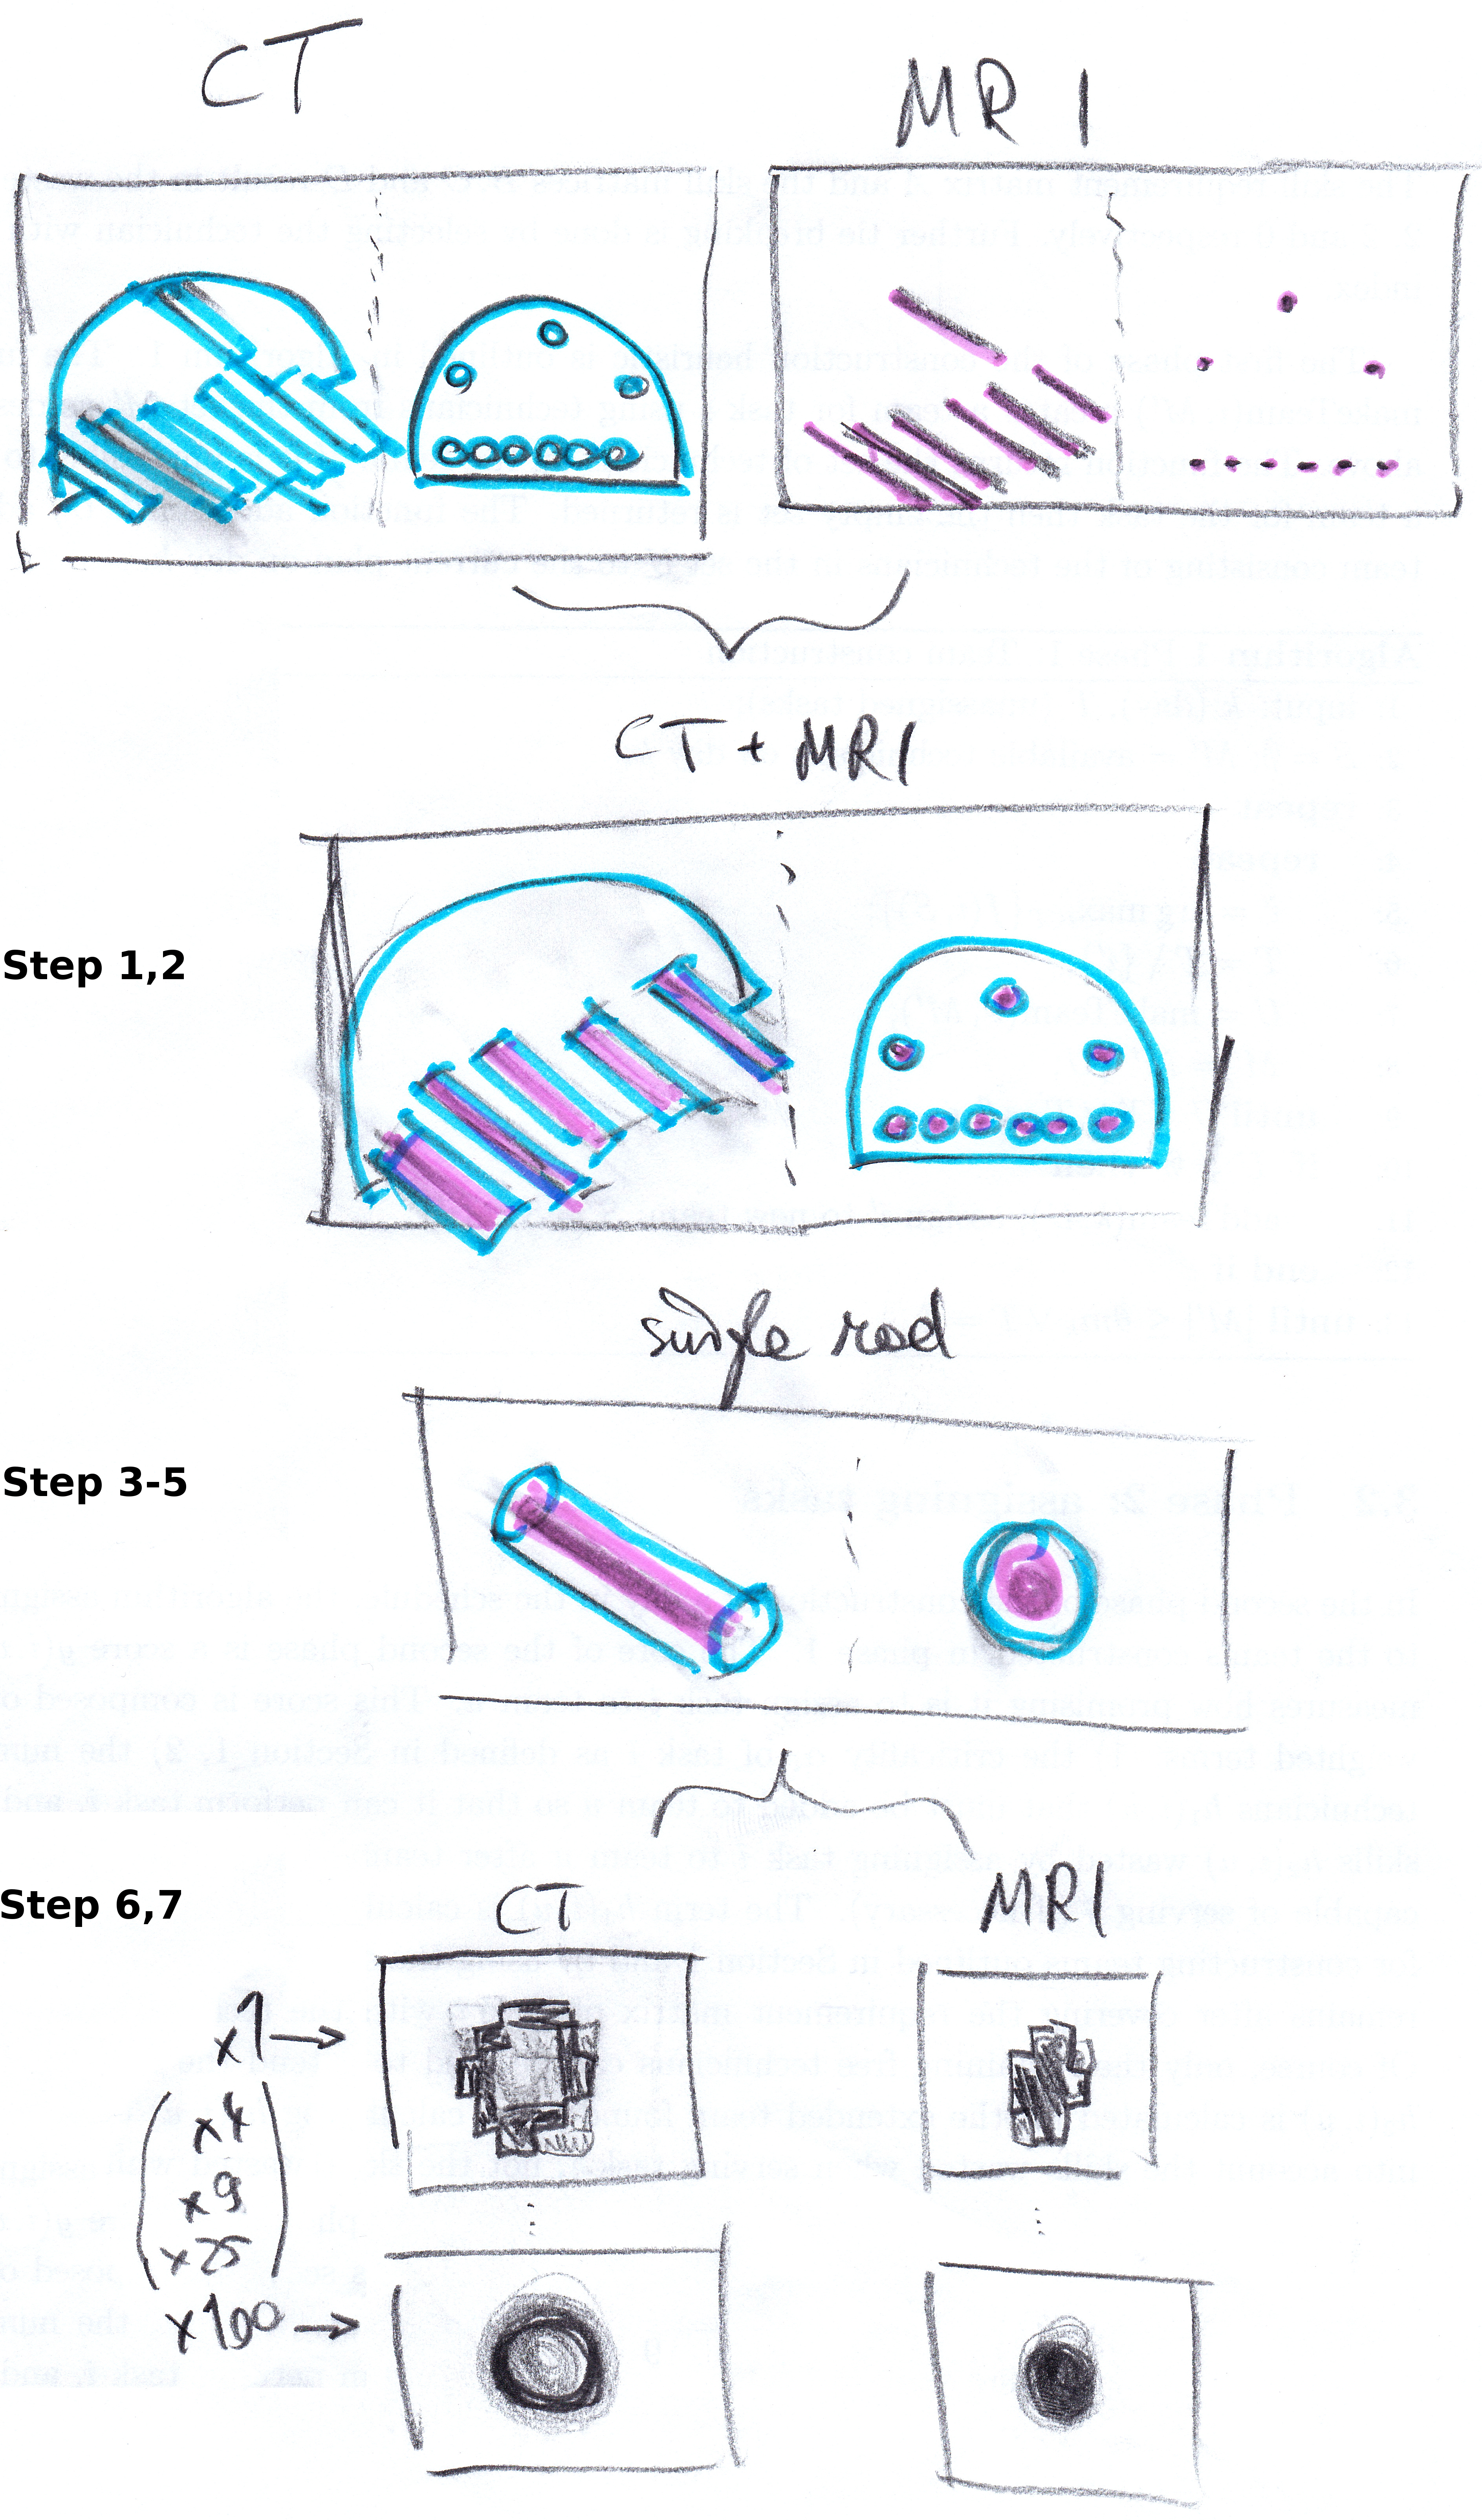
\includegraphics[width=0.8\textwidth]{algorithm/data_prep.jpg}
\caption{Steps performed before analysing data with script}
\label{fig:data_prep}
\end{figure}

After this procedure a number of data sets based on the original CT and MRI was available, which all had the same number of slices along the z-axis parallel to the phantom's rods.
Each pair (CT+MRI) has the same pixel spacing (/resolution) in x and y direction.
See table \ref{tab:spacing} for more details.
Figure \ref{fig:resample} depicts 3 CT/MRI scans of a single rod (axial) with different resolutions.
``x1'' stands for the original CT scan resolution (MRI resampled to match).
``x4'' is a resolution resulting in 1 pixel being split in 4 smaller pixels, ``x9'' in 9, and so on and so forth.
For better visibility, images shown as figures in this work are printed with inverted colours.
Dark pixels have a high density/intensity value, white pixels are equivalent to air (low density/intensity).

\begin{table}[!htb]
\centering
\begin{tabular}{l|l|l|l}
resample factor  & z (not affected) &  y (same as x) & x \\
\toprule
x1     & 0.60 & 0.98	& 0.98	\\
x4     & 0.60 & 0.49	& 0.49	\\
x9     & 0.60 & 0.33	& 0.33	\\
% x16    & 0.60 & 0.244	& 0.24	\\
x25    & 0.60 & 0.2 	& 0.2	\\
x100   & 0.60 & 0.2 	& 0.1
\end{tabular}
\caption{pixel Spacing (rounded values) [$mm$]}
\label{tab:spacing}
\end{table}


\begin{figure}[!thb]
  \begin{subfigure}[b]{0.32\textwidth}
    \includegraphics[scale=.11]{slicer3D/profiles/CT_x1.png}
    \caption{CT x1}
    \label{fig:CT_x1}
  \end{subfigure}
  \hfill
  \begin{subfigure}[b]{0.32\textwidth}
    \includegraphics[scale=.11]{slicer3D/profiles/CT_x9.png}
    \caption{CT x9}
    \label{fig:CT_x9}
  \end{subfigure}
    \hfill
  \begin{subfigure}[b]{0.32\textwidth}
    \includegraphics[scale=.11]{slicer3D/profiles/CT_x100.png}
    \caption{CT x100}
    \label{fig:CT_x100}
  \end{subfigure}
  \begin{subfigure}[b]{0.32\textwidth}
    \includegraphics[scale=.11]{slicer3D/profiles/MR_x1.png}
    \caption{MRI x1}
    \label{fig:MRI_x1}
  \end{subfigure}
  \hfill
  \begin{subfigure}[b]{0.32\textwidth}
    \includegraphics[scale=.11]{slicer3D/profiles/MR_x9.png}
    \caption{MRI x9}
    \label{fig:MRI_x9}
  \end{subfigure}
    \hfill
  \begin{subfigure}[b]{0.32\textwidth}
    \includegraphics[scale=.11]{slicer3D/profiles/MR_x100.png}
    \caption{MRI x100}
    \label{fig:MRI_x100}
  \end{subfigure}
  \caption{CT/MRI: axial image of single rod, filling \#5  (inverted colours)}
  \label{fig:resample}
\end{figure}
\clearpage


\subsection{Capabilities}

The developed software tool is not able to automatically detect individual rods shown in a CT or MRI scan.
Instead the acquired 3D images have to be cropped to depict only a single rod.

The python script can:
\begin{itemize}
 \item denoise the image data
 \item accepts coordinates to be used as seeds, enabling it to separate bright areas which are not connected ('masking' might be used as future method to automatically detect individual rods
 \item calculate the centroid coordinates along the rod, used to
 \item measure the local distortion
  \subitem location shift
  \subitem dice coefficient (roundness/deformation)
 \item plot individual rod slices
  \subitem overlaying one or two centroid coordinates
  \subitem and save it as ``.png'' file
 \item change the pixel values to reflect the distortion occurring along a rod (visualisation)
 \item write the calculated numbers to a ``.txt'' file
\end{itemize}

\subsection{Measuring distortion}

Two phenomena were chosen to reflect the amount of distortion occurring in MRI scans:

\begin{enumerate}[label=\textbf{\arabic*)}]
 \item location shift (``warp'')
 \item deformation (deviation from circular profile ``DC'')
\end{enumerate}

Since the rods have a cylindrical shape, distortion can only be assessed in radial direction.
To make calculations easier, the z-coordinate was put parallel to the rods, x and y radial.
Ideally, each slice (z = const.) should depict the bright circular profile of the liquid (+ plastic rod in CT) surrounded by black (air).
To calculate the location shift between rods shown in CT and MRI, the coordinates of the centre of mass (COM) were subtracted.
The location difference in each slice is saved as an array.
Additionally, the absolute value of the coordinate shift (warpMagnitude) could be calculated.

% image of COM shift

The dice-coefficient ``DC'' (also known as Sorensen-Index) was chosen as indicator for the deviation from a circular profile. Again this value was calculated for every slice using either the CT or MRI scans.

To get a idea of the occurring distortion one should look at both the absolute value of coordinate shift and the dice-coefficient (DC).
The DC ranges from 0 to 1. A value of 1 indicates a perfect circular shape. A low DC on the other hand could be caused by many things such as:
little overlap (e.g. a ring or crescent shape); a very dark image hindering delineation of rod from background; a small circle with a radius close to a only a few pixels.


% A proposed third indicator combining warp magnitude and the DC:
% $warpDC = warpMagnitude * (1-DC)$

\subsection{Calculation: dice-coefficient (DC)}

The dice coefficient or Sorensen index \cite{MedPy_dc-doc} is defined as:

\begin{align}
DC = \frac{2 |A \, \cap \, B|}{|A| + |B|}
\end{align}

The implementation into python is based on the open source python package ``Medpy''. \cite{MedPy} A part of it's module called ``metric'' was adapted. \cite{MedPy_dc-code}
All pixels above a certain threshold will be counted as input A. The reference B is a circle whose midpoint is placed at the centre of mass (COM).

The calculation of the DC is done by comparing an binary image to a circle. The position of the circle's centre and its radius is highly influencing the outcome.
Both the circle's centre and its radius were varied during the distortion assessment.


\subsection{Calculation: center of mass (COM)}

The calculation of the COM is done with help of the ``scipy'' python package.
It's module ``ndimage'' contains the function ``$center\_of\_mass()$'', which returns the COM's coordinates of a given input array.
The values assigned to voxels in CT images lie in the range from -1024 HU (air) to around 200 HU (plastic rod).
Before a meaningful result can be obtained, the values need to be shifted to be $>$ 0.
Additionally, only pixels representing the rod or the liquid should be used for the calculation.
Otherwise the almost black voxels surrounding the rod would influence the result.
This error could be observed especially if the rod is not placed in the exact middle of the scan.
As described earlier, the plastic rod is only visible in CT images. On the MRI scans solely the liquid containded in the rods is shown.
Therefore, rods appear to be smaller on the MRI data.
To find the relevant pixels two algorithms were developed:

\begin{description}
 \item[1] calculating the number of pixels based on rod size
 \item[2] finding a COM resulting in good DC
\end{description}

\textit{\textbf{add 1:}}
The inner ($4mm$) and outer ($8mm$) diameter of the rods are known. So is the \textit{pixel spacing} which represents the equivalent size of a voxel in $mm$.
Calculating the number of pixels which make up the more or less circular profile of the rod in each slice is calculated as follows:

\begin{align}
 pixelNumber = (radius^2 \cdot \pi) \, / \, (spacing^2)
\end{align}

For CT images $radius = 4mm$, in MRI scans $radius = 2mm$. $spacing$ is the pixel spacing in x and y direction.
Next the pixels are sorted by brightness. The top $pixelNumber$ pixels are then used to calculate the COM.

\textit{\textbf{add 2:}}
This algorithm is an iteration method.
First it looks at the whole range of possible pixelNumbers, from $0\%$ to $100\%$.
It starts off by assuming that $50\%$ is a reasonable guess for the number of pixels that show the rod and calculates the corresponding DC value.
To find out whether more or less pixels would result in a better DC, it chooses two new guesses:
One halfway from the lower limit ($0\%$) to its current guess ($50\%$) which is:

\begin{align}
 \frac{0+50}{2}=25\% 
\end{align}

and one halfway from the upper limit ($100\%$) to its current guess ($50\%$) which is:
 
\begin{align}
 \frac{100+50}{2}=75\%
\end{align}
 
Now the corresponding DC values are calculated and compared.
If the lower percentage yields a better DC, the upper half of the range will be neglected in the next iteration, the upper limit becomes the former guess ($50\%$).
If the higher percentage yields a better DC, the lower half of the range will be neglected in the next iteration, the lower limit becomes the former guess ($50\%$).

Now in the second iteration, the range has become smaller and the next guess will be set to be exactly in the middle.
If, for example, the DC for $25\%$ was higher, the next guess will be $25\%$, because the new range goes from $0\%$ to $50\%$.
In that case, DC values for the lower half of the range ($12,5\%$) and the upper half ($18,5\%$) will be calculated and compared.
If, for example, the DC for $18,5\%$ was higher, the next guess will then be $18,5\%$, because the new range goes from $25\%$ to $50\%$.
The iteration continues until new steps yield no better DCs or a set number of steps has been performed.

After the iteration process, the algorithm will return the COM which resulted in the best DC.
Figure \ref{fig:COM_iteration} shows the DC values found in the course of the iteration method
Figure \ref{fig:COM_iteration_flow} summarises the algorithm.

\todo{flowchart for algorithms (send handwritten draft to Piotr)}
\clearpage

\begin{figure}[!thb]
  \begin{subfigure}[b]{1\textwidth}
    \includegraphics[scale=0.7]{python/iteration_COM/CT_x100_iteration_COM.png}
    \caption{CT x100, (4 steps lead to best result)}
    \label{fig:CT_x100_iteration}
  \end{subfigure}
  \begin{subfigure}[b]{1\textwidth}
    \includegraphics[scale=0.7]{python/iteration_COM/MR_x100_iteration_COM.png}
     \caption{MR x100, (15 step performed)}
     \label{fig:MR_x100_iteration}
  \end{subfigure}
  \caption{COM iteration method}
  \label{fig:COM_iteration}
\end{figure}

% image of COM shift


\chapter{Results}
% o Present all results here
% o No discussion, no interpretation, no evaluation etc.
% o Figures / Tables
%  Use wisely
%  Consult your supervisor about what to present
%  put very large and detailed tables rather in the appendix
%  put source code in appendix
% o Do not write down all data from table in text, but put them in relation to each other
% o Help reader to understand tables & graphs and highlight important and/or interesting data
% o Present an assessment of uncertainties

On the second day of working with the filled rods the one containing liquid \textbf{\#6} broke (leakage).
It happened when delicately knocking it against on the table while standing upright.
This was intended to mobilise bubbles that sticked to the wall and make them travel vertically to on end of the rod. (see table \ref{tab:bubbles})
The plastic stopper on the lower end came loose.
The rod containing filling \textbf{\#6} was not replaced.
Consequently, all CT/MRI images used to asses signal intensities of the tested solutions show only 16 rods.

\section{Obtained MRI and CT scans}
Figure \ref{fig:coronal} shows a coronal view of the 16 rods filled with the tested liquids and a reference rod on either side.
In Figure \ref{fig:coronal_MR} a trapped air bubble is clearly visible at the lower half of rod \#5.
Figure \ref{fig:axial} shows an axial view of the tested rods and some surrounding rods.
In figure \ref{fig:axial_MR} a water filled plastic bottle placed in the middle of the phantom is also visible.
This was necessary, because the MRI scanner needs sufficient signal for shimming prior to the start of imaging.
Without the bottle, the limited number of rods used for this scan would not have created enough signal.
During a future distortion assessment where all available rods (over 300) are used, they will result in the required signal strength on their own.
 
\begin{figure}[!tbp]
  \begin{subfigure}[b]{\textwidth}
    \includegraphics[width=\textwidth]{slicer3D/full_phantom/coronal_CT_cropped-arrow.png}
    \caption{CT: The periodic black lines in upper and lower part of image (indicated with arrows) depict the plastic panes and their holes from above; The faint line across upper end of rods shows adhesive tape used to hold the rods in place; In rod \#17 an air bubble is clearly visible close to the upper end.}
    \label{fig:coronal_CT}
  \end{subfigure}
  \begin{subfigure}[b]{1\textwidth}
    \includegraphics[width=1\textwidth]{slicer3D/full_phantom/coronal_MR_cropped.png}
    \caption{MR: The rods appear to be thinner than in the CT scan, because only the liquid filling is visible. The tested liquids result in different signal intensity (brightness); all plastic parts (rods and panes) are not visible; there is a trapped air bubble visible in rod \#5.}
    \label{fig:coronal_MR}
  \end{subfigure}
  \caption{Coronal CT/MRI (inverted colours; same scale; cropped images) images of 16 rods (tested liquids, numbering starting from the right, \#6 excluded) + 2 reference rods (filled with water) on the sides.}
  \label{fig:coronal}
\end{figure}

\begin{figure}[!tbp]
  \begin{subfigure}[b]{\textwidth}
    \includegraphics[width=\textwidth]{slicer3D/full_phantom/axial_CT_rods-arrow.png}
    \caption{CT: The black bars visible just above the 16 tested rods, at the very top, and to the sides show plastic parts of the phantom holding it together. The faint grey line running below the tested rods represents the table on which the phantom was positioned during imaging.}
    \label{fig:axial_CT_rods}
  \end{subfigure}
  \begin{subfigure}[b]{\textwidth}
    \includegraphics[width=\textwidth]{slicer3D/full_phantom/axial_MR-arrow.png}
    \caption{MRI: The black circle in the centre depicts a water bottle which was placed in the middle of the phantom (necessary for MRI scanner to start imaging).}
    \label{fig:axial_MR}
  \end{subfigure}
  \caption{axial CT/MRI (inverted colours, same scale) images of the 16 rods filled with tested liquids (numbering starting from the right, \#6 excluded); surrounded by reference rods (filled with water) and one empty rod (marked with arrow) which is not visible on the MRI scan}
  \label{fig:axial}
\end{figure}


\section{Tested solutions}

\subsection{Visibility on CT/MRI scans}

It should be noticed that in the CT image there is little difference in brightness between the tested liquids.
The plastic rods themselves result in brighter pixels than any of the tested solutions.

On MRI scans most liquids had a mean and a max brightness value above $1000$ (see table \ref{tab:visibility}).\\
Only \textbf{\#1}, \textbf{\#9}, \textbf{\#10}, \& \textbf{\#17} resulted in significantly less signal (below < $1000$).


\begin{table}[!htb]
\centering
\begin{tabular}{@{}l|lllll@{}}
\toprule
No. & Min  & Max  & Mean   & Median & $\sigma$ \\ \midrule
1   & 182  & 371  & 288    & 269    & 69,8     \\
2   & 1044 & 1921 & 1443,8 & 1405   & 312,9    \\
3   & 941  & 2075 & 1451,2 & 1394,5 & 413,2    \\
4   & 1176 & 1709 & 1440   & 1437,5 & 232,5    \\
5   & 1125 & 2111 & 1583,8 & 1549,5 & 355      \\
7   & 971  & 2241 & 1466,8 & 1316   & 471,2    \\
8   & 1459 & 1947 & 1704   & 1705   & 180,5    \\
9   & 385  & 584  & 486,8  & 489    & 93       \\
10  & 247  & 502  & 343,6  & 266    & 111      \\
11  & 830  & 1268 & 1036,2 & 1023,5 & 163,2    \\
12  & 1158 & 2211 & 1648,8 & 1613   & 394,2    \\
13  & 836  & 1657 & 1146,8 & 1047   & 321,2    \\
14  & 800  & 2062 & 1383   & 1335   & 473,1    \\
15  & 1156 & 1829 & 1476,2 & 1460   & 272,7    \\
16  & 1102 & 1967 & 1509   & 1483,5 & 325,8    \\
17  & 356  & 938  & 629,6  & 602    & 223,6    \\ \bottomrule
\end{tabular}
\caption{liquid visibility on MRI scan}
\label{tab:visibility}
\end{table}

\clearpage

\subsection{Mechanical properties of solutions}
\label{sec:sol-mech}

The liquids were filled in a rod each and observed for several months.
Number \textbf{\#14} could be injected without problems, the solution remained fluid even after reaching room temperature.
Number \textbf{\#15} on the other hand changed to a gel like consistence and clogged the injection tube at the quickly after the rod was filled.
The tube could not be used again.

Each rod was free of bubbles directly after sealing.
All rods containing water based solutions contained some air after 2 months and the amount of liquid continued to decrease further (see table \ref{tab:bubbles}).
After 6 months the volume of air further increased (proportionally to the behaviour observed until then).
Figure \ref{fig:bubbles} shows the rods after a time of over 6 months.
In some of the tested rods, the occurring air bubbles would stick to the wall.
Only after gently hitting the rod they would start moving.
Knowing the inner diameter $d$ of the rods and measuring the length $l$ of trapped air bubbles, their volume can be estimated:

\begin{align}
 V = \frac{d^2}{4}\cdot \pi \cdot l
\end{align}

\begin{table}[]
\centering
\begin{tabular}{l|lc|lc|lc}
    & \multicolumn{2}{c}{\textit{after 1 day}} 	& \multicolumn{2}{c}{\textit{after 2 days}}	& \multicolumn{2}{c}{\textit{after 1 week}}	\\ 
No. & bubbles	& hit req.	& bubbles 	& hit req.	& bubbles 	& hit req.	\\
\toprule
\#1   & yes	& no		& no		&		& no		&		\\
\#2   & yes	& yes		& no		&		& no		&		\\
\#3   & yes	& yes		& no		&		& no		&		\\
\#4   & yes	& yes		& no		&		& no		&		\\
\#5   & yes	& no		& yes		& no		& no		&		\\
\#6   & yes	& no		& \multicolumn{4}{l}{-----------------\textit{ rod was leaking }------------------}	\\
\#7   & yes	& no		& yes		& no		& yes		& no		\\
\#8   & no	&		& no		&		& no		&		\\
\#9   & no	&		& no		&		& no		&		\\
\#10  & no$^1$	&		& yes		& yes		& yes		& yes		\\
\#11  & no	&		& yes,		& \textit{sticked to wall} &	 yes	& yes\\
\#12  & yes	& yes		& yes,		& \textit{sticked to wall} &	 yes	& yes\\
\#13  & yes	& yes		& yes,		& \textit{sticked to wall} &	 yes	& yes\\
\#14  & no	&   		& yes		& no		& yes		& yes		\\
\#15  & no	&   		& no		&		& no		&		\\
\#16  & no	&   		& no		&		& no		&		\\
\#17  & no	&   		& no		&		& no		&		\\
\bottomrule
\end{tabular}
\begin{tabular}{l|lr}
\multicolumn{3}{c}{}								\\
& \multicolumn{2}{c}{\textit{after 2 months}}					\\ 
No. & length of trapped bubble $l$ [$mm$] 	& approx. volume $V$ [$mm^3$]	\\
\toprule
\#1   & 2					& 25.13				\\
\#2   & 1.8					& 22.62				\\
\#3   & 1+1 (air blockage, at lower end)	& 25.13				\\
\#4   & 4					& 50.27				\\
\#5   & 1.5 (many small bubbles)		& 18.85				\\
\#6   & \multicolumn{2}{c}{-----------------------------\textit{ rod was leaking }------------------------------}\\
\#7   & 2 (many small bubbles)			& 25.13				\\
\#8   & 2.3					& 28.90				\\
\#9   & 3					& 37.70				\\
\#10  & 2.4					& 30.16				\\
\#11  & 2					& 25.13				\\
\#12  & 2					& 25.13				\\
\#13  & 2.3					& 28.90				\\
\#14  & 1.5+0.5 (big immobile bubble, at center)	& 25.13				\\
\#15  & 3.4 (agar gel dried)			& 42.73				\\
\#16  & 0					& 0.00				\\
\#17  & 0.5					& 6.28				\\
\bottomrule
\end{tabular}
\caption{Observations regarding the mechanical properties of the tested solutions.}
\label{tab:bubbles}
\end{table}


While adding generic washing soap (\textbf{\#5}, \textbf{\#6} and \textbf{\#7}) did not hinder air bubbles from forming, it significantly improved their mobility.
Not only did they move quickly when the rod was tilted, large quantities of air also did not block the entire diameter of the rod.
Instead they formed large but cohesive bubbles that could be moved to one end of the rod easily and at no point sticked to the plastic wall.

The ascorbic acid present in \textbf{\#8} (concentration of $0.36 \; g/L$ corresponds to approx. $0.00204 \; mol/L$), \textbf{\#9} ($3.6 g/L$), and \textbf{\#10} ($36 g/L$) seemed to have held back the formation of air bubbles for up to one week.
After two months of observation, however, the rods also contained some air.
It should be noted that all three liquids turned brown, the colour being more saturated for higher concentrations of ascorbic acid.

The rods filled with Primovist (\textbf{\#11} to \textbf{\#13}) were filled with some air bubbles after at least two days.
Moreover, the bubbles sticked to the walls of the rod and only shaking it violently made them move to one side of the rod.

It took more than a week until the rod containing the low concentration of agar (\textbf{\#14}) contained an air bubble.
The viscous consistency made it impossible to coerce it to either end of the rod.
Liquid \textbf{\#15} on the other hand did not form bubbles at the middle of the rod, but seemed to have dried starting at the end with the plastic stopper.

\begin{figure}[tbh!]
\centering
\includegraphics[width=1\linewidth]{photo/rods_bubbles_crop.jpg}
\caption{Most tested rods (except \#5,\#6 and \#16) after more than 6 months.}
\label{fig:bubbles}
\end{figure}


\begin{figure}[tbh!]
\centering
\includegraphics[width=1\linewidth]{photo/bubbles_cuso.png}
\caption{Rod \#5 showed some bubbles after 2 months.}
\label{fig:bubbles_cuso}
\end{figure}

\begin{figure}[tbh!]
\centering
\includegraphics[width=1\linewidth]{photo/oil.png}
\caption{Rod \#16 contained no bubbles after more than 6 months.}
\label{fig:bubbles_oil}
\end{figure}

\section{Distortion assessment}
%As described later, resolution might influence the efficiency of the distortion assessment.#	
%Therefore all calculations were done with the original resolution and interpolated images that have a higher resolution.

\subsection{rod \#5}

The first scans were not only used to asses the brightness of the different solutions, but also to calculate occurring distortion.
As an example, the rod containing liquid \#5 was analysed.
Table \ref{tab:spit-out-5} shows the most interesting areas of the rod.


The obtained dice coefficient varies not only because of the circle's centre and the radius, it also depends on the images resolution.
Figure \ref{fig:CT_dc} and \ref{fig:MR_dc} show the DC (optimised) obtained using CT and MRI scans over resample rate.

 \begin{table}[p]
    \centering
    \rotatebox{90}{
      \begin{minipage}{\textheight}\footnotesize
        \centering
 \begin{tabular}{rr||lll|lll||lll|lll}
 slice	& dist & $warp_x$ & $warp_y$ & $warpM$ & $DC_{CT}$ & $DC_{MR}$ & $DC_{MR(CT-COM)}$ & $warp_x^*$ & $warp_y^*$ & $warpM^*$ & $DC^*_{CT}$	& $DC^*_{MR}$ & $DC^*_{MR(CT-COM)}$\\ \hline
 0      & -183 & -0.1046 & -1.115  & 1.1199 & 0.981  & 0.846  & 0.5982 & -0.1104 & -1.0595 & 1.0653 & 0.9906 & 0.9477 & 0.5982 \\
 1      & -182 & -0.1205 & -1.1132 & 1.1197 & 0.9832 & 0.8551 & 0.6037 & -0.1245 & -1.0514 & 1.0588 & 0.9906 & 0.9487 & 0.6037 \\
 2      & -181 & -0.1278 & -1.1107 & 1.1181 & 0.9831 & 0.8678 & 0.6109 & -0.1313 & -1.0485 & 1.0567 & 0.9846 & 0.948  & 0.5813 \\
 :      &      &         &         &        &        &        &        &         &         &        &        &        &        \\
 \hline
 :      &      &         &         &        &        &        &        &         &         &        &        &        &        \\
 171    & -12  & 0.0025  & -0.6891 & 0.6891 & 0.9847 & 0.9412 & 0.7571 & -0.0313 & -0.6969 & 0.6976 & 0.9869 & 0.9451 & 0.7571 \\
 172    & -11  & 0.0089  & -0.6825 & 0.6825 & 0.9865 & 0.9412 & 0.7571 & -0.0272 & -0.7012 & 0.7017 & 0.9822 & 0.9458 & 0.7571 \\
 173    & -10  & -1      & -1      & -1     & -1     & 0.9409 & -1     & -1      & -1      & -1     & -1     & 0.946  & -1     \\
 174    & -9   & -1      & -1      & -1     & -1     & 0.9413 & -1     & -1      & -1      & -1     & -1     & 0.9458 & -1     \\
 :      & :    & :       & :       & :      & :      &        &        & :       & :       & :      &        &        &        \\
 \hline &      &         &         &        &        &        &        &         &         &        &        &        &        \\
 :      & :    & :       & :       & :      & :      &        &        & :       & :       & :      &        &        &        \\
 192    & 9    & -1      & -1      & -1     & -1     & 0.9464 & -1     & -1      & -1      & -1     & -1     & 0.95   & -1     \\
 193    & 10   & -1      & -1      & -1     & -1     & 0.9479 & -1     & -1      & -1      & -1     & -1     & 0.9504 & -1     \\
 194    & 11   & 0.0379  & -0.709  & 0.71   & 0.989  & 0.9484 & 0.7649 & 0.0028  & -0.7153 & 0.7153 & 0.9805 & 0.9496 & 0.7649 \\
 195    & 12   & 0.0364  & -0.7048 & 0.7058 & 0.989  & 0.948  & 0.7661 & 0.0033  & -0.7156 & 0.7156 & 0.9821 & 0.9498 & 0.7661 \\
 :      &      &         &         &        &        &        &        &         &         &        &        &        &        \\
 \hline
 :      &      &         &         &        &        &        &        &         &         &        &        &        &        \\
 301    & 118  & 0.2997  & -0.8702 & 0.9204 & 0.9785 & 0.4295 & 0.3962 & 0.1128  & -0.8025 & 0.8104 & 0.9841 & 0.8861 & 0.3962 \\
 302    & 119  & 0.3943  & -1.1317 & 1.1984 & 0.9818 & 0.1453 & 0.1423 & 0.1073  & -0.8906 & 0.8971 & 0.9841 & 0.8666 & 0.1423 \\
 303    & 120  & -1      & -1      & -1     & 0.9822 & -1     & 0      & 0.1066  & -1.0077 & 1.0133 & 0.9841 & 0.8317 & 0      \\
 304    & 121  & -1      & -1      & -1     & 0.9832 & -1     & 0      & 0.0896  & -1.1827 & 1.1861 & 0.9857 & 0.7845 & 0      \\
 305    & 122  & -1      & -1      & -1     & 0.9828 & -1     & 0      & 0.0852  & -1.4164 & 1.419  & 0.9854 & 0.7153 & 0      \\
 306    & 123  & -1      & -1      & -1     & 0.9824 & -1     & 0      & 0.0769  & -1.5832 & 1.5851 & 0.9849 & 0.6758 & 0      \\
 307    & 124  & -1      & -1      & -1     & 0.9833 & -1     & 0      & 0.0788  & -1.5436 & 1.5456 & 0.9851 & 0.7156 & 0      \\
 308    & 125  & -1      & -1      & -1     & 0.982  & -1     & 0      & 0.0826  & -1.5257 & 1.5279 & 0.9862 & 0.7501 & 0      \\
 309    & 126  & -1      & -1      & -1     & 0.9837 & -1     & 0      & 0.0868  & -1.48   & 1.4826 & 0.9859 & 0.7831 & 0      \\
 310    & 127  & 0.3786  & -2.0028 & 2.0383 & 0.9805 & 0.0754 & 0.011  & 0.0718  & -1.4467 & 1.4485 & 0.9865 & 0.8135 & 0.011  \\
 311    & 128  & 0.3434  & -1.9836 & 2.0131 & 0.9837 & 0.1648 & 0.0629 & 0.0775  & -1.4081 & 1.4102 & 0.9862 & 0.8422 & 0.0434 \\
 :      &      &         &         &        &        &        &        &         &         &        &        &        &        \\
 \hline
 :      &      &         &         &        &        &        &        &         &         &        &        &        &        \\
 393    & 210  & 0.1083  & -0.2563 & 0.2783 & 0.9819 & 0.9334 & 0.8938 & 0.0968  & -0.2638 & 0.281  & 0.9863 & 0.9613 & 0.8938 \\
 394    & 211  & 0.1147  & -0.263  & 0.2869 & 0.9828 & 0.932  & 0.8932 & 0.0993  & -0.2653 & 0.2832 & 0.9852 & 0.9617 & 0.8932 \\
 395    & 212  & 0.1214  & -0.2454 & 0.2738 & 0.9836 & 0.9338 & 0.8984 & 0.1041  & -0.2532 & 0.2738 & 0.9839 & 0.9621 & 0.8958
 \end{tabular}
        \caption{rod \#5: script generated data}
        \label{tab:spit-out-5}
      \end{minipage}
    }
  \end{table}
 


\begin{figure}[!tbp]
  \begin{subfigure}[b]{0.32\textwidth}
    \includegraphics[scale=0.55]{python/ph2/centroid/CT_x100@0_centroids.png}
    \caption{CT @ 0}
    \label{fig:CT_x100_centroids@0}
  \end{subfigure}
  \begin{subfigure}[b]{0.32\textwidth}
    \includegraphics[scale=0.55]{python/ph2/centroid/CT_x100@150_centroids.png}
    \caption{CT @ 150}
    \label{fig:CT_x100_centroids@150}
  \end{subfigure}
  \begin{subfigure}[b]{0.32\textwidth}
    \includegraphics[scale=0.55]{python/ph2/centroid/CT_x100@304_centroids.png}
    \caption{CT @ 304}
    \label{fig:CT_x100_centroids@304}
  \end{subfigure}
  \begin{subfigure}[b]{0.32\textwidth}
    \includegraphics[scale=0.55]{python/ph2/centroid/MR_x100@0_centroids.png}
    \caption{MRI @ 0}
    \label{fig:MR_x100_centroids@0}
  \end{subfigure}
  \begin{subfigure}[b]{0.32\textwidth}
    \includegraphics[scale=0.55]{python/ph2/centroid/MR_x100@150_centroids.png}
    \caption{MRI @ 150}
    \label{fig:MR_x100_centroids@150}
  \end{subfigure}
  \begin{subfigure}[b]{0.32\textwidth}
    \includegraphics[scale=0.55]{python/ph2/centroid/MR_x100@304_centroids.png}
    \caption{MRI @ 304}
    \label{fig:MR_x100_centroids@304}
  \end{subfigure}
  \caption{MRI x100 scan of rod filled with \#5 (true colours). The dark blue dot represents the MRI centroid, the bright red dot represents the CT centroid.
  			\\ Slice 150 is located approximately at the isocentre, 0 on the very end of the image, 304 on the other but also close to an air bubble.}
  \label{fig:MR_x100_centroids}
\end{figure}


\begin{figure}[!bp]
  \centering
  \includegraphics[scale=0.6]{python/ph2/warp/warpXY_x100_iter.png}
  \caption{Rod \#5: warp XY [$mm$] (iteration method), CT-MRI x100}
  \label{fig:ph2_warpXY_x100}
\end{figure}

\begin{figure}[!tp]
    \centering
    \includegraphics[scale=0.6]{python/ph2/warp/warpMagnitude_x100_iter.png}
    \caption{Rod \#5: warp Magnitude [$mm$] (iteration method), CT-MRI x100}
    \label{fig:ph2_warpMagnitude_x100}
\end{figure}

\begin{figure}[!bp]
    \centering
    \includegraphics[scale=0.6]{python/ph2/dice/ph2_DC_x100_iter.png}
    \caption{Rod \#5: DC (iteration method) for CT \& MRI \& MRI (using CT COM)}
    \label{fig:ph2_DC_x100}
\end{figure}

\begin{figure}[!bp]
  \centering
  \includegraphics[scale=0.6]{python/ph2/dice/ph2_CT_DC-15radii_simple_close.png}
  \caption{Rod \#5: CT DC of varied radii \& resolutions}
  \label{fig:ph2_CT_DC-15iter}
\end{figure}

\begin{figure}[!tbp]
  \centering
    \includegraphics[scale=0.6]{python/ph2/dice/ph2_MR_DC-15radii_simple.png}
    \caption{Rod \#5: MRI DC of varied radii \& resolutions}
    \label{fig:ph2_MR_DC-15iter}
\end{figure}

\begin{figure}[!tbp]
      \centering
    \includegraphics[scale=0.6]{python/ph2/dice/ph2_MR_DC-15radii_CT_COM_simple_close.png}
    \caption{Rod \#5: MRI DC of varied radii \& resolutions (using CT-COM)}
    \label{fig:ph2_MR_CT-COM_DC-15iter}
\end{figure}

\clearpage



\subsection{rod \#17}

After deciding which of the possible liquids might be a suitable choice for future use of the phantom, another set of MRI/CT scan was taken.
This second data set shows the rod conatining liquid \#17.
Again it was analysed using the developed script.
Table \ref{tab:spit-out-17} shows the most interesting areas of the rod.

\begin{table}[p]
   \centering
   \rotatebox{90}{
     \begin{minipage}{\textheight}\footnotesize
       \centering
\begin{tabular}{rr||lll|lll||lll|lll}
slice	& dist & $warp_x$ & $warp_y$ & $warpM$ & $DC_{CT}$ & $DC_{MR}$ & $DC_{MR(CT-COM)}$ & $warp_x^*$ & $warp_y^*$ & $warpM^*$ & $DC^*_{CT}$	& $DC^*_{MR}$ & $DC^*_{MR(CT-COM)}$\\ \hline
0       & -361 & 2.9415  & 0.4286  & 2.9725        & 0.967  & 0.0286 & 0.0077         & 3.2985   & 0.8734   & 3.4122         & 0.9406  & 0.603   & 0.0131          \\
1       & -360 & 2.94    & 0.4294  & 2.9712        & 0.9698 & 0.0286 & 0.0077         & 3.2943   & 0.8677   & 3.4067         & 0.9396  & 0.604   & 0.0131          \\
2       & -359 & 2.9441  & 0.4224  & 2.9742        & 0.9717 & 0.0338 & 0.0092         & 3.2666   & 0.8416   & 3.3732         & 0.9416  & 0.6014  & 0.0145          \\
:       &      &         &         &               &        &        &                &          &          &                &         &         &                 \\
\hline
:       &      &         &         &               &        &        &                &          &          &                &         &         &                 \\
351     & -10  & -0.2049 & -0.0356 & 0.208         & 0.9854 & 0.9307 & 0.9045         & -0.2709  & -0.1155  & 0.2945         & 0.9907  & 0.932   & 0.9045          \\
352     & -9   & -0.2217 & -0.0174 & 0.2223        & 0.9853 & 0.9307 & 0.9056         & -0.2813  & -0.0996  & 0.2984         & 0.9832  & 0.9313  & 0.9056          \\
353     & -8   & -1      & -1      & -1            & -1     & 0.9302 & -1             & -1       & -1       & -1             & -1      & 0.9304  & -1              \\
354     & -7   & -1      & -1      & -1            & -1     & 0.9296 & -1             & -1       & -1       & -1             & -1      & 0.9295  & -1              \\
355     & -6   & -1      & -1      & -1            & -1     & 0.9276 & -1             & -1       & -1       & -1             & -1      & 0.9262  & -1              \\
356     & -5   & -1      & -1      & -1            & -1     & 0.9253 & -1             & -1       & -1       & -1             & -1      & 0.9187  & -1              \\
357     & -4   & -1      & -1      & -1            & -1     & 0.9198 & -1             & -1       & -1       & -1             & -1      & 0.9185  & -1              \\
358     & -3   & -1      & -1      & -1            & -1     & 0.9174 & -1             & -1       & -1       & -1             & -1      & 0.9178  & -1              \\
359     & -2   & -1      & -1      & -1            & -1     & 0.9142 & -1             & -1       & -1       & -1             & -1      & 0.9179  & -1              \\
360     & -1   & -1      & -1      & -1            & -1     & 0.912  & -1             & -1       & -1       & -1             & -1      & 0.9184  & -1              \\
361     & 0    & -1      & -1      & -1            & -1     & 0.909  & -1             & -1       & -1       & -1             & -1      & 0.9079  & -1              \\
362     & 1    & -1      & -1      & -1            & -1     & 0.8999 & -1             & -1       & -1       & -1             & -1      & 0.9055  & -1              \\
363     & 2    & -1      & -1      & -1            & -1     & 0.9007 & -1             & -1       & -1       & -1             & -1      & 0.9031  & -1              \\
364     & 3    & -1      & -1      & -1            & -1     & 0.9011 & -1             & -1       & -1       & -1             & -1      & 0.9008  & -1              \\
365     & 4    & -1      & -1      & -1            & -1     & 0.9012 & -1             & -1       & -1       & -1             & -1      & 0.8981  & -1              \\
366     & 5    & -1      & -1      & -1            & -1     & 0.9028 & -1             & -1       & -1       & -1             & -1      & 0.8961  & -1              \\
367     & 6    & -1      & -1      & -1            & -1     & 0.9052 & -1             & -1       & -1       & -1             & -1      & 0.9006  & -1              \\
368     & 7    & -1      & -1      & -1            & -1     & 0.908  & -1             & -1       & -1       & -1             & -1      & 0.9045  & -1              \\
369     & 8    & -1      & -1      & -1            & -1     & 0.9109 & -1             & -1       & -1       & -1             & -1      & 0.9024  & -1              \\
370     & 9    & -1      & -1      & -1            & -1     & 0.9138 & -1             & -1       & -1       & -1             & -1      & 0.9057  & -1              \\
371     & 10   & -1      & -1      & -1            & -1     & 0.9159 & -1             & -1       & -1       & -1             & -1      & 0.9116  & -1              \\
372     & 11   & -1      & -1      & -1            & -1     & 0.9216 & -1             & -1       & -1       & -1             & -1      & 0.9177  & -1              \\
373     & 12   & -1      & -1      & -1            & -1     & 0.9233 & -1             & -1       & -1       & -1             & -1      & 0.9219  & -1              \\
374     & 13   & -0.2506 & 0.1242  & 0.2797        & 0.9859 & 0.9284 & 0.9142         & -0.2553  & 0.0875   & 0.2699         & 0.9899  & 0.9284  & 0.9142          \\
375     & 14   & -0.2181 & 0.1166  & 0.2473        & 0.9838 & 0.9354 & 0.9207         & -0.2258  & 0.091    & 0.2434         & 0.9926  & 0.9287  & 0.9207          \\
:       &      &         &         &               &        &        &                &          &          &                &         &         &                 \\
\hline
:       &      &         &         &               &        &        &                &          &          &                &         &         &                 \\
609     & 248  & 3.0734  & 0.7814  & 3.1712        & 0.9803 & 0.9316 & 0.363          & 3.0791   & 0.9091   & 3.2105         & 0.9825  & 0.9225  & 0.363           \\
610     & 249  & 3.1422  & 0.7546  & 3.2315        & 0.9796 & 0.9345 & 0.3446         & 3.1281   & 0.8819   & 3.2501         & 0.9822  & 0.9329  & 0.3446          \\
611     & 250  & 3.2214  & 0.7399  & 3.3053        & 0.9832 & 0.9363 & 0.3085         & 3.1826   & 0.8566   & 3.2958         & 0.9828  & 0.9358  & 0.325          
\end{tabular}
       \caption{rod \#17: script generated data}
       \label{tab:spit-out-17}
     \end{minipage}
   }
 \end{table}

\begin{figure}[!bp]
  \centering
  \includegraphics[scale=0.6]{python/ph3_v2/warp/ph3_MR_v2_x100_warpXY_iter.png}
  \caption{Rod \#17: warp XY [$mm$] (iteration method), CT-MRI x100}
  \label{fig:ph3_warpXY_x100}
\end{figure}

\begin{figure}[!tp]
    \centering
    \includegraphics[scale=0.6]{python/ph3_v2/warp/ph3_MR_v2_x100_warpMagnitude_iter.png}
    \caption{Rod \#17: warp Magnitude [$mm$] (iteration method), CT-MRI x100}
    \label{fig:ph3_warpMagnitude_x100}
\end{figure}

\begin{figure}[!bp]
     \centering
     \includegraphics[scale=0.6]{python/ph3_v2/dice/ph3_MR_v2_x100_DC_iter.png}
     \caption{Rod \#17: DC (iteration method) for CT \& MRI \& MRI (using CT COM)}
     \label{fig:ph3_DC_x100}
\end{figure}

\todo{PIOTR: create colour coded images}

% \begin{figure}[!tbp]
%   \begin{subfigure}[b]{\textwidth}
%     \centering
%     \includegraphics[scale=0.65]{python/ph2/dice/CT_dice-comparison_fast-51iter.png}
%     \caption{CT: x1, x4, x9, x16, x25, x100}
%     \label{fig:MR_dice-comp}
%   \end{subfigure}
%   \begin{subfigure}[b]{\textwidth}
%     \centering
%     \includegraphics[scale=0.65]{python/ph2/dice/MR_dice-comparison_fast-51iter.png}
%     \caption{MRI: x1, x4, x9, x16, x25, x100}
%     \label{fig:MR_dice_comp}
%   \end{subfigure}
%   \caption{}
%   \label{fig:dice_com}
% \end{figure}

% image of COM shift
%This kind of comments need to go to the dicussion. As mentioned above here you report on the results. So the numbers, tables and images. You can write the the rod X was better vissible than Y. One iquid waseasier to fill than other. But what you thing is more useful and why (considering all pros and cons) you need to put in the dicussion. That is why it is called discussion :)



\chapter{Discussion}
% o Interpretation of results, putting them in context with literature
% o Discuss only results which were presented in the results section and do not repeat them one by one
% o Which impacts have your results on the scientific community?
% o provide an assessment of the weaknesses and strengths of your work
% o At least 5 pages

\section{Phantom design}

To be able to assess the spacial distortion of an MRI scan, a rigid object with known dimensions needs to be scanned so the cross referencing to the ground truth can be performed.
Such phantoms are commercially available, but often expensive and designed for a specific calibration protocol.
Some institutions build their own to fulfil exactly the requirements of a given application.
The scanner used at the AKH is a relatively rare model, which is why no off-the-shelf phantom that would fit its coil is available.

A previously used phantom did not fill the whole FOV, while at the same time weighing about 45kg.
This was due to the fact that it resembled a cuboid water tank with a thin plastic rod construction inside.
As the peripheral zones of the FOV are those where distortion is most pronounced, a bigger phantom was needed to assess those regions.
The new design deals with both issues effectively.
Due to the underlying physics, plastics are not visible in MR scans, but CT scans visualize them. 
See figure \ref{fig:sagittal_comparison} for a comparison (MRI/CT visibility).
Therefore, it was decided to use plastic rods with a suitable fluid filling.
Such a liquid should be easily produced, non-toxic, and yielding sufficient signal in MRI scans.

Commercially available phantoms often resemble water filled tanks containing plastic grids as a reference.
This design results in stronger signal, but exceeds practical weight.
There are few brands offering solutions utilising liquid fiducial markers in the shape of pellets.
They are arranged in a regular pattern surrounded by air or plastic.
The AKH's design however relies on replaceable rods, which makes it a novelty.

\subsection{Observed issues}

Interestingly, all water based solutions seemed to have evaporated partly.
As the rod filled with liquid \textbf{\#15} has dried starting at the end with the plastic stopper, it seems likely that, at least in this particular case, the plastic stopper did not effectively close the rod.
It might also be that the rod itself does not prevent volatile liquids from escaping slowly.
This was tested in a small experiment where an empty, closed rod was placed underwater.
After some time water bubbles formed along its wall.
An airtight container might have lead to other conclusions regarding the formation of air bubbles.
It is hard to tell if they were caused by evaporation only or if dissolved gases played a role, too.
Whatever the reasons are, the use of water based liquids seems to be suboptimal.
Despite this, the observed behaviour will still be discussed as a future airtight phantom design might benefit from any drawn conclusion.

\section{Tested solutions}

For measuring the position of the rods in the CT scans, the plastic rods without filling would be enough already.
Hollow plastic rods would not be visible on the MRI scans, though.
That is why the visibility of the liquids on CT is not important at all.
From now on 'signal (strength)' or 'visibility' will refer to MRI scans only (see table \ref{tab:visibility}).

\subsection{Thoughts about choosing possible candidates}

The selection of solutions tested were chosen for a number of reasons:
\begin{enumerate}[label=\textbf{\arabic*.}]
\item Generally, imaging techniques aims for a high signal-to-noise ratio. Therefore, Liquids resulting in brighter pixels are favoured.
\item The amount of gas in the rods should be minimised.
\item If air bubbles form, tilting the entire phantom slightly should be enough to move them to one side. The FOV of the MRI scanner is too small to show the entire phantom anyway.
\item Most tested fluids are based on water, because this makes them easy to empty and clean.
They could then be filled again with a different liquid if needed.
\item Preferably, the components which are chosen to be used for the entire phantom should be non-toxic if not swallowed.
\end{enumerate}

\vspace{1cm}

Rod \textbf{\#1} was filled with plain distilled water an intended to be used only as a reference.
It was clear from the beginning that it would not result in high signal and was never considered a possible filling.

\subsubsection{Aiming for high SNR}
To achieve a better SNR, liquids \textbf{\#2} to \textbf{\#10} and \textbf{\#14} to \textbf{\#15} are based on a solution of sodium chloride ($NaCl$ concentration of $0.36 \, g/L$) and copper(II) sulfate pentahydrate ($CuSO_4\cdot5H_2O$ concentration of $1.96 \, g/L$ as suggested by AAPM MR Subcommittee \cite{Jackson2009};  \textbf{\#3} and \textbf{\#4} contain double and ten-fold the concentration) in distilled water.
Most of these liquids resulted in an about 5 times brighter signal than plain distilled water.
Regarding the toxicity of $CuSO_4\cdot5H_2O$, the minimum dose to have caused acute toxic effects in humans is reported to be $11 mg/Kg$.
%As the concentration of $CuSO_4\cdot5H_2O$ is only $1.96 \, g/L$, even a young patient of 4 years and $15kg$ would need to drink more than 80mL to reach that threshold.
%Also, ingestion usually leads to vomiting triggered by its irritating effect on the gastrointestinal tract, which would stop further (more severe) toxic effects from happening.
%Keeping the scanner bed clean and checking the phantom for leakage before and after use should be sufficient to prevent an intoxication.
% http://pmep.cce.cornell.edu/profiles/extoxnet/carbaryl-dicrotophos/copper-sulfate-ext.html#2

\vspace{1cm}

Primovist (\textbf{\#11} to \textbf{\#13}) is a common contrast agent used for MRI scans \cite{VanBeers2012, Rohrer, primovist} intended to yield an even stronger signal than $CuSO_4\cdot5H_2O$ based liquids.
The major drawback is its tendency to separate from the water and stick to the phantom's wall.
This results in low signal at the centre and high signal along the wall, which would not pose a problem in itself, but as the liquid forms bubbles it is not guaranteed that the walls would be covered homogeneously.
The uneven distribution might result in wrong calculations, especially if the software tool is not programmed to cope with this behaviour.
At the same time the removal would be hardly possible.

\subsubsection{Handling dissolved gas}
Unfortunately, dissolved gases may eventually leave the liquid and form air bubbles.

To improve the mobility of trapped air bubbles, generic washing-up soap was added (\textbf{\#5}, \textbf{\#6}, and \textbf{\#7}; suggestion by Data Spectrum Corporation \cite{bubbles}).
%The smallest amount of 1 g/L was already enough to result in sufficient mobility and an even lower concentration might also be acceptable.
The higher concentrations of soap were tested as reference.
%Interestingly, the rod filled with this solution contained the least amount of gas after 2 months.
If the liquid should happen to leak from the rod, the relatively low concentration of soap would not add to its toxicity.
%The visibility recorded was among the higher candidates, too.
For those reasons, and because the liquid is cheap and easy to produce, it appears to be a promising candidate.

\vspace{1cm}

Liquids \textbf{\#8} ($0.36 g/L$), \textbf{\#9} ($3.6 g/L$), and \textbf{\#10} ($36 g/L$) contain ascorbic acid.
Adding this was supposed to reduce forming of air bubbles by binding dissolved oxygen and eventually degrade to dehydro-ascorbic acid and water.
The amount suggested by \cite{Abtahi2008, Bodannes1979} is $0.00204 \; mol/L$ which corresponds to approx. ($0.36 g/L$).

\vspace{1cm}

In an attempt to limit the forming of gas, \textit{agar} was used in solutions \textbf{\#14} and \textbf{\#15}.
Agar and agarose are commonly used as basic reference material for MRI phantoms \cite{BuccioliniCiraolo1989, Mathur-DeVre1985}
%Since the produced gel cannot be removed from the rods as easily as liquid candidates, and forming air bubbles were also not moving, agar is not suited for this phantom.

\subsubsection{Non water-based liquids}
As an alternative 2 oils were proposed.
Since air is not soluble in oil, once a rod is completely with oil, no air bubbles should form.
Yet, oil is not as easily removed from a rod as a water based liquid.
At the same time, it might not be necessary to ever replace the oil.
Once filled, the rods could be used until the surrounding plastic breaks or starts leaking.
Using vegetable oil would be a non-toxic solution, but has been ruled out as a filling from the beginning, because it would eventually rot.
Mineral oil on the other hand does not rot, however, it might be toxic if consumed.
%As the generic motor (\textbf{\#16}) oil resulted in the highest signal intensity of all candidates it seems to be a good alternative to water based liquids.
%The silicon oil (\textbf{\#17}) on, the other side, had a low signal compared to most candidates and is therefore not suited.


\subsection{Choosing a promising candidate}
As all rods containing water continued to lose liquid due to evaporation, only the early forming of air bubbles might indicate whether solutions effectively hinder dissolved gases to result in trapped air bubbles.
Apart from the solutions containing ascorbic acid (\textbf{\#8} ($0.36 g/L$), \textbf{\#9} ($3.6 g/L$)) all water based liquids produced some air bubbles after at least two days (see table \ref{sec:sol-mech}).
Considering the low visibility of \textbf{\#9}, the only suitable water based liquid capable of staying free from air bubbles might be \textbf{\#8}.
At the same time, long-term observations performed in an airtight container might have shown that even \textbf{\#8} only delays the process.
In the case of the used rods, such a conclusion cannot be drawn with certainty.

The rod containing the highest concentration of ascorbic acid showed a yellow colouring, caused by dehydroascorbic acid which is the result of a oxygenation process.
However, as the high concentration in \textbf{\#9} and \textbf{\#10} led to a radical reduction in signal with the tested MRI sequence, this solutions is not considered a suitable filling anyway.

Primovist (\textbf{\#11} to \textbf{\#13}) lead to a good signal, but its limited mobility of air bubbles; its tendency to accumulate along the wall; and the difficulty of cleaning the rods rule it out as a candidate.

If the forming of  a small amount of gas is not considered a problem, adding soap appears to be a reasonable solution.
The smallest tested amount of soap (\textbf{\#5}, 1 g/L) was already enough to result in sufficient mobility of air bubbles, and an even lower concentration might also be acceptable.
Interestingly, the rod filled with this solution contained the least amount of gas after 2 months, but this might be because the particular rod closed better than the others.
The visibility recorded was among the higher candidates, too.
For those reasons, and because the liquid is cheap and easy to produce, it is a promising candidate.

Solutions containing \textit{agar} (\textbf{\#14} and \textbf{\#15}) are even harder to remove from rods if not impossible.
As they might lead to air bubbles, too, which cannot be moved to either side of the rod, agar is not suited for this phantom.

Finally, the synthetic motor (\textbf{\#16}) oil resulted in the highest signal intensity of all candidates.
Besides the question of its toxicity, it seems to be a good alternative to water based liquids.
The silicon oil (\textbf{\#17}) on, the other side, had a low signal compared to most candidates and is therefore not suited.


\section{Distortion}

\subsection{Calculation Methods}
\texttt{DC} and warp values calculated with the simple or iteration method do not differ much.
Moreover, both methods choose very similar thresholds for their calculations (see appendix)
As the simple method uses additional information on the rod's true dimension, it is supposed to yield accurate, reliable results.
The iteration process, oblivious to the imaging modality, supports this claim as it produces very similar numbers.


At the moment it does not take into account the steepness of the DC curve.
In some cases it might yield better results if tweaked slightly.
This leads to the left hand side close to very low percentages to be neglected sometimes.
This happens when the perfect guess lies roughly in the middle of the current range, but a little bit to the left.
Because the slope is steeper on the left (close to 0\%), a value representing the left hand side (also close to 0\%) yields a much lower result than the value on the right hand side (flat slope).
This should be taken into account during further improvement of the method.

Figure \ref{fig:MR_x100_centroids} visualises the centroid shift in significant slices.
It is clearly visible that the shift is bigger at one end of the rod (slice 0) compared to a slice close to the middle (slice 150).
Furthermore, the 

\subsection{Irregularities}
\todo{rewrite}
In the case of a slice located at a plastic pane, the CT image will be mostly very bright, as the plastic results in a high intensity.
Consequently, this slice will be marked as irregular as the average brightness differs greatly from the reference slice's.
However, the MRI scan will not show such a increase in brightness at that location, as plastic is not visible for the MRI scanner.
Here the MRI data will not be marked as irregular, provided there is no other cause for a change in brightness, like an air bubble.
Such an absence of liquid would result in a drastic decrease of brightness and result in an irregular slice.
In CT, on the other hand, an air bubble would hardly make a difference, as the surrounding plastic is far brighter than the contained liquid.

\subsection{DC calculation}
\label{sec:discussion_DC}

\subsection{COM calculation}
\todo{rewrite}



%Gnerally this graphs are OK, but we discused before you left that there is need to comment of what we actually see on them, as you explained that to me. Also we dicussed that you could add a figure showing a particular slice on which a certain problem occures (why is the extra-high distortion dettected: a bubble or artefact). 

%We also talked that the XY axes have to properly called, so on X distance from the middle instead of the slice etc. Based on this descriptoion we could write smth clever in the discussion.  

To get a idea of the occurring distortion one should look at both the absolute value of coordinate shift and the dice-coefficient (DC).
An air bubble might lead to a incorrect COM.
Without looking at the dice-coefficient it is hard to tell why this distortion only appears to be present in a few slices.
If both indicators show unexpected local irregularities, a conclusion might be easier to draw.



\todo{discuss what is visible on the graphs in results section}
\todo{interpret data table spit out by script}
\todo{scale of distortion, bigger on the sides as expected}
\todo{only x,y direction. future design needs objects going from left to right, too.}

\chapter{Conclusion and Outlook}
% o Summary of study
%  Most important results and their meaning/impact and conclusions
%  Outlook
%  open questions
%  Next steps

Successfully found a suitable solution/liquid.
Imaging sequences are ready.
Distortion assessment can be performed using the generated tool, however, it needs to be implemented on more general scale to be able to measure the distortion for all the rods automatically
    
\section{Future improvement of software tool}

The developed tool took a simplified approach to the problem by looking only at a single rod.
Future improvements should enable the software to take into account all the rods automatically.
This could be done by a autotrace function which detects individual rods and applies the already implemented algorithms to each of them separately. 


\chapter*{Appendix}

The current version of the python script 'FunITK.py' with all functions described in this thesis used to calculate the presented numbers is available at: \url{https://github.com/cyberspeck/mri-for-rt/blob/master/scripts}

The data of the cropped images showing rod \#5 and \#16, the created '.txt' and '.mha' files are stored at: \url{https://github.com/cyberspeck/mri-for-rt/tree/master/data}



\cleardoublepage
%\pagenumbering{roman} \setcounter{page}{1}
%\nocite{*}
\printbibliography
%\input{thanks.tex}

%\appendix
%\input{appendix01.tex}

\end{document}